\documentclass[namedreferences,hyperref,optionalrh]{spr-sola}
\usepackage{graphicx}        % For eps figures, newer & more powerfull
%\usepackage{amssymb}        % useful mathematical symbols
\usepackage[dvipsnames]{xcolor}           % For color text: \color command
%\usepackage{color}           % For color text: \color command
%\usepackage{breakurl}                         % For breaking URLs easily trough lines in DVI mode
\def\UrlFont{\rm}                        % define the fonts for the URLs

% General definitions
% please place your own definitions here and don't use \def but
% \newcommand{}{} or 
% \renewcommand{}{} if it is already defined in LaTeX

\newcommand{\BibTeX}{\textsc{Bib}\TeX}
\newcommand{\etal}{et al.}

% Definitions for equations
\renewcommand{\vec}[1]{{\mathbfit #1}}
\newcommand{\deriv}[2]{\frac{{\mathrm d} #1}{{\mathrm d} #2}}
\newcommand{\rmd}{{\ \mathrm d}}
\newcommand{\uvec}[1]{\hat{\mathbf #1}}
\newcommand{\pder}[2]{\f{\partial #1}{\partial #2}}
\newcommand{\grad}{{\bf \nabla}}
\newcommand{\curl}{{\bf \nabla}\times}
\newcommand{\vol}{{\mathcal V}}
\newcommand{\bndry}{{\mathcal S}}
\newcommand{\dv}{~{\mathrm d}^3 x}
\newcommand{\da}{~{\mathrm d}^2 x}
\newcommand{\dl}{~{\mathrm d} l}
\newcommand{\dt}{~{\mathrm d}t}
\newcommand{\intv}{\int_{\vol}^{}}
\newcommand{\inta}{\int_{\bndry}^{}}
\newcommand{\avec}{\vec A}
\newcommand{\ap}{\vec A_p}

\newcommand{\bb}{\vec B}
\newcommand{\jj}{\vec j}
\newcommand{\rr}{\vec r}
\newcommand{\xx}{\vec x}

% text with colors
\newcommand{\p}[1]{{\color{magenta}{#1}}}
\renewcommand{\mp}[1]{{\color{blue}{#1}}}
\newcommand{\mpc}[1]{{\bf \color{blue}{[Mariano comment: #1]}}}
%\newcommand{\pc}[1]{{\color{green}{P comment: #1}}}
\newcommand{\pc}[1]{{\color{ForestGreen}{P comment: #1}}}
%\newcommand{\pr}[1]{{\color{orange}{P remove: #1}}}
\newcommand{\cm}[1]{{\color{orange}{#1}}}

% Definitions for the journal names
\newcommand{\adv}{{\it Adv. Space Res.}} 
\newcommand{\annG}{{\it Ann. Geophys.}} 
\newcommand{\aap}{{\it Astron. Astrophys.}}
\newcommand{\aaps}{{\it Astron. Astrophys. Suppl.}}
\newcommand{\aapr}{{\it Astron. Astrophys. Rev.}}
\newcommand{\ag}{{\it Ann. Geophys.}}
\newcommand{\aj}{{\it Astron. J.}} 
\newcommand{\apj}{{\it Astrophys. J.}}
\newcommand{\apjl}{{\it Astrophys. J. Lett.}}
\newcommand{\apss}{{\it Astrophys. Space Sci.}} 
\newcommand{\cjaa}{{\it Chin. J. Astron. Astrophys.}} 
\newcommand{\gafd}{{\it Geophys. Astrophys. Fluid Dyn.}}
\newcommand{\grl}{{\it Geophys. Res. Lett.}}
\newcommand{\ijga}{{\it Int. J. Geomagn. Aeron.}}
\newcommand{\jastp}{{\it J. Atmos. Solar-Terr. Phys.}} 
\newcommand{\jgr}{{\it J. Geophys. Res.}}
\newcommand{\mnras}{{\it Mon. Not. R. Astron. Soc.}}
\newcommand{\nat}{{\it Nature}}
\newcommand{\pasp}{{\it Publ. Astron. Soc. Pac.}}
\newcommand{\pasj}{{\it Publ. Astron. Soc. Japan}}
\newcommand{\pre}{{\it Phys. Rev. E}}
\newcommand{\solphys}{{\it Sol. Phys.}}
\newcommand{\sovast}{{\it Soviet  Astron.}} 
\newcommand{\ssr}{{\it Space Sci. Rev.}} 
\chardef\us=`\_

%%%%%%%%%%%%%%%%%%%%%%%%%%%%%%%%%%%%%%%%%%%%%%%%%%%%%%%%%%%%%%%%%%
\begin{document}

\begin{frontmatter}
\title{Tilt Angle of Bipolar Active Regions from Solar Cycle 23}

\author[addressref={aff1},email={mpoisson@iafe.uba.ar}]{\inits{M.}\fnm{Mariano}~\snm{Poisson}\orcid{0000-0002-4300-0954}}
%\author[addressref=aff1,email={e-mail.b@mail.com}]{\inits{F.}\fnm{First~Names}~\snm{Surname~Author-b}}
%\author[addressref=aff2,corref,email={e-mail.c@mail.com}]{\inits{F.}\fnm{First~Names}~\snm{Surname~Author-c}\orcid{987-654-3210}}
%\author[addressref=aff3]{\inits{T.}\fnm{First~Names}~\snm{Surname~Author-d}}
%\author{\inits{}\fnm{}~\lnm{}\orcid{}}
%   NOTE:  Just one corresponding author [corref]
\address[id=aff1]{Instituto de Astronomía y Física del Espacio, CONICET-UBA,CABA, Argentina.}
%\address[id=aff2]{L'observatoire de Paris, LESIA, Meudon, France}
%\address[id=aff3]{Third affiliation and address}

\runningauthor{Author-a et al.}
\runningtitle{Tilt Angle of Bipolar ARs}

\begin{abstract}

Active regions (ARs) are the photospheric manifestation of the emergence of magnetic flux ropes (FRs) formed in the solar interior. A key parameter in an AR evolution is its tilt angle, defined as the inclination of the AR polarity axis with respect to the solar equator, which plays a central role in flux-transport dynamo models that explain the cyclic transformation of toroidal to poloidal magnetic fields. However, measuring the tilt angle is affected by projection effects, such as magnetic tongues, particularly during the AR emergence phase.
In this work, we analyze tilt angle estimations for 126 bipolar ARs from Solar Cycle 23 using two methodologies: (1) the conventional magnetic barycenter method, which calculates the bipole axis based on the centroids of the polarities, and (2) a Bayesian FR method, which employs synthetic magnetograms simulating the emergence of a twisted toroidal flux tube to fit observed AR magnetograms via Bayesian inference. The Bayesian FR method accounts for projection effects and provides a more accurate estimation of the intrinsic tilt, especially during the early stages of emergence {when magnetic tongues are most extended}.
We perform a statistical analysis of tilt angle evolution, showing that the Bayesian FR method reduces tilt dispersion providing a more reliable estimation of Joy’s law. 

\end{abstract}
\keywords{Active Regions, Magnetic Fields;
                 Active Regions, Models;Magnetic fields, Photosphere}
\end{frontmatter}
%-------------------------------------------------

\section{Introduction}
     \label{S-Introduction} 
     
Active regions (ARs) are fundamental manifestations of the Sun’s magnetic activity and play a crucial role in shaping the dynamics of the solar cycle. Their evolution is directly linked to solar eruptions, coronal mass ejections, and space weather phenomena \citep{schrijver2000, toriumi2019}. Understanding the formation and magnetic properties of ARs has been a long-standing focus in solar physics, driving advances in observational techniques and theoretical modeling.

A key mechanism underlying AR formation is the emergence of magnetic flux ropes (FRs)—twisted bundles of magnetic field lines formed in the solar interior. These structures rise buoyantly through the convection zone due to a combination of magnetic pressure and reduced plasma density \citep{fan2001, cheung2014}. The degree of twist in an FR influences its stability and likelihood of producing solar eruptions, with highly twisted FRs being more prone to destabilization \citep{liu2016, torok2018}.

In line-of-sight magnetograms, FR twist manifests as elongated polarity extensions known as magnetic tongues.. These features, which arise due to the azimuthal component of the FR magnetic field, are most prominent during the early stages of AR emergence \citep{luoni2011, Poisson16}. Their presence alters the observed magnetic flux distribution, affecting the determination of key AR properties, including the tilt angle.

The tilt angle of an AR—defined as the angle between the line connecting the centroids of opposite polarity regions and the solar equator—is a critical parameter in dynamo models, as it plays a fundamental role in regulating the solar magnetic cycle \citep{stenflo2012}. The statistical tendency for the tilt angle to increase with latitude, known as Joy’s law, serves as a key input for flux-transport models that simulate large-scale solar magnetic field evolution \citep{Hale19, dasi2010, Yeates2023}.

Determining the tilt angle with precision is challenging due to the complexity of AR emergence. Magnetic tongues, in particular, shift the apparent positions of polarity centroids, introducing systematic biases in tilt angle measurements \citep{Poisson22}. Correcting for these distortions is essential to refine tilt angle estimates and to investigate deviations from Joy’s law, such as the observed suppression of tilt at high flux values \citep{jiang2020}.

In \citet{Poisson16}, a statistical study of bipolar ARs from Solar Cycle 23 demonstrated that magnetic tongues serve as a proxy for FR twist and significantly impact tilt angle measurements. The study highlighted the necessity of correcting for these effects, especially when discrepancies arise between different tilt estimation methods.

Building on this, \citet{Poisson20a} introduced the Core Field Fit Estimator (CoFFe), a method designed to estimate the intrinsic inclination of FRs. This technique effectively mitigates the impact of magnetic tongues, leading to more reliable tilt angle measurements. A subsequent comparison between CoFFe and other methods, such as those based on flux-weighted polarity centroids and white-light observations, revealed substantial differences in derived tilt angles \citep{Poisson2020b}.

Expanding upon these efforts, \citet{Poisson22} applied Bayesian inference to model FR emergence using line-of-sight magnetograms. This approach, which approximates the FR as a half-torus, was validated against synthetic data and a single observed AR, demonstrating improved robustness in recovering key FR parameters. However, the method was limited to single-magnetogram analyses, leaving room for further refinement.

In \citet{Poisson24}, the Bayesian method was extended to incorporate temporal coherence, allowing inferred parameters to evolve smoothly over time. This refinement provided a dynamic representation of the emergence process and enabled a more detailed exploration of parameter constraints. The study identified optimal prior selections and parameter space configurations, advancing our understanding of FR evolution.

In this article, we extend previous analyses by applying Bayesian inference to a large dataset of 126 bipolar ARs from Solar Cycle 23. Our objectives are threefold: (1) refine tilt angle corrections, particularly during early emergence stages, addressing biases introduced by magnetic tongues. (2) Evaluate the impact of these corrections on Joy’s law and assess their implications for solar dynamo models. (3) Compare Bayesian-inferred tilt angles with traditional methods, such as those based on magnetic barycenters, and analyze discrepancies. 
Section~\ref{S-data} introduces the dataset, Section~\ref{S-method} summarizes the Bayesian method, Section~\ref{S-comparetilt} compares tilt estimates from both methods, and Section~\ref{S-conclusions} summarizes our findings and their implications for solar cycle modeling.

%Section~\ref{S-data} describes the dataset and preprocessing of line-of-sight magnetograms. Section~\ref{S-bayes} outlines the Bayesian modeling approach, emphasizing its robustness across the full dataset. Section~\ref{S-method-tilt} presents a comparative analysis of tilt angle estimates and their evolution. Finally, Section~\ref{S-conclusions} summarizes our findings and discusses their broader implications.


%% Figure Butterfly
%
 \begin{figure} 
 \centerline{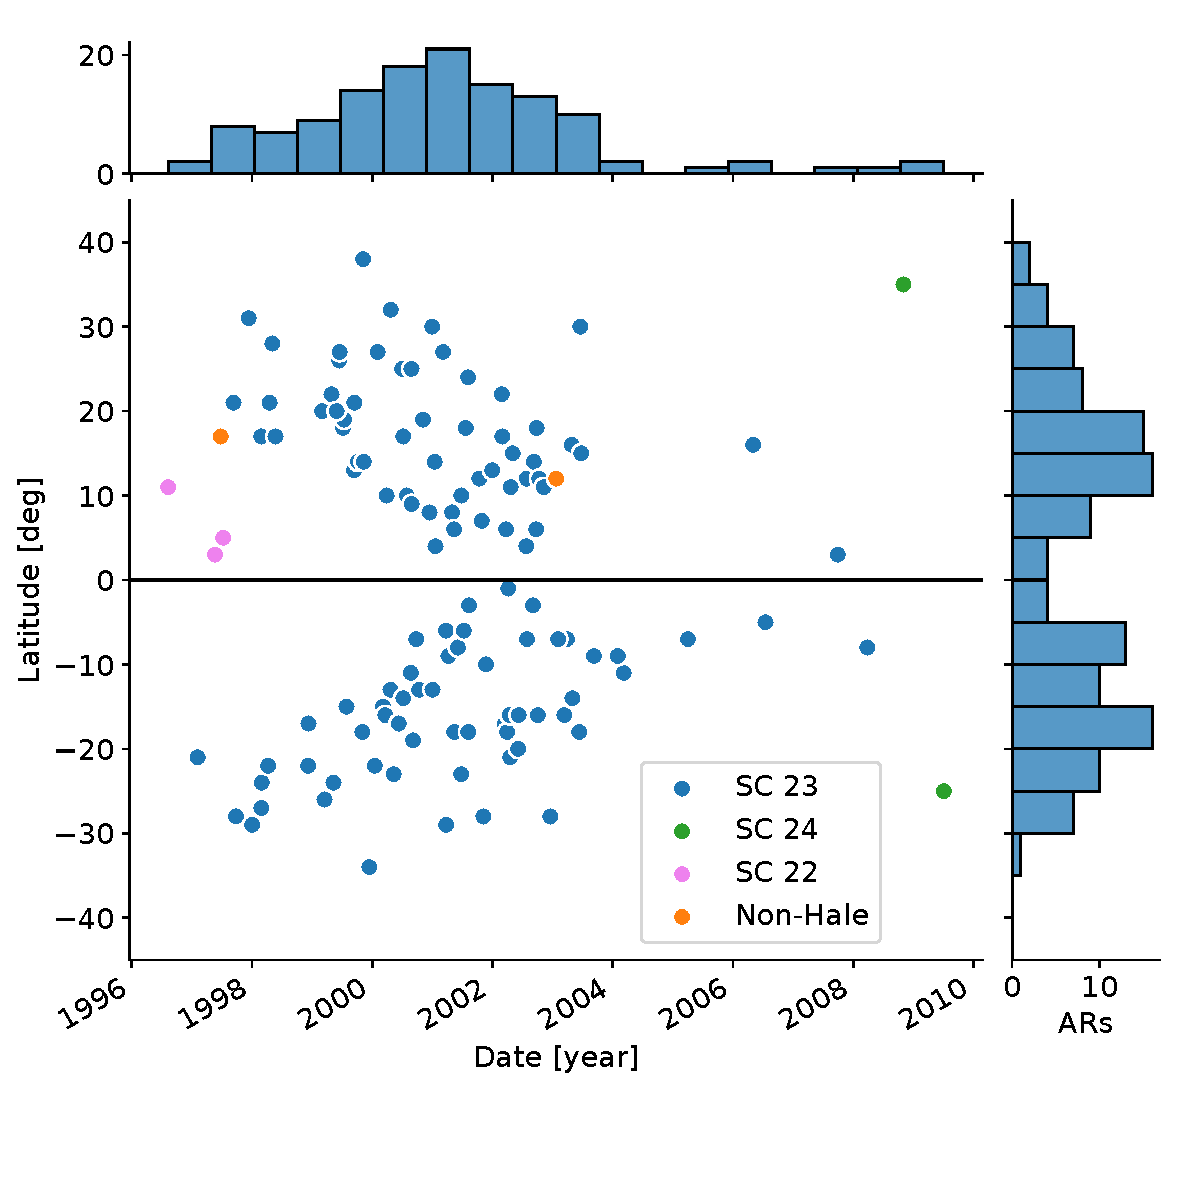
\includegraphics[width=0.9\textwidth,clip=]{./plots/butterfly.pdf}}
 \caption{Butterfly diagram of the 126 bipolar ARs in our sample. Blue dots correspond to ARs emerging in Solar Cycle 23. Violet and green dots correspond to ARs from Cycles 22 and 24, respectively, while orange dots mark the non-Hale bipoles. The top histogram shows the temporal distribution of AR emergences (bin size 6 months), and the right histogram shows their latitudinal distribution (bin size $5^\circ$).}\label{fig:butt}
 \end{figure}

\section{AR selection and Data Processing} %%%%%%%%%%%%%%
  \label{S-data}

We analyzed the evolution of 126 bipolar ARs using line-of-sight (LOS) magnetograms from the Michelson Doppler Imager \citep[MDI;][]{Scherrer95} onboard the Solar and Heliospheric Observatory (SOHO). This dataset spans almost the full duration of Solar Cycle 23 (July 1996–January 2010). MDI produced full-disk magnetograms at a 96-minute cadence by averaging either one-minute or five-minute magnetograms, with flux density errors of 16 G and 9 G per pixel, respectively \citep[][]{Liu04}. Each day, 15 magnetograms were available, with a resolution of 1024 × 1024 pixels and a spatial scale of $1.98^{\prime\prime}$ per pixel.

Figure~\ref{fig:butt} displays the latitude and emergence time of the 126 bipolar ARs from our selected dataset. The ARs were selected based on three main criteria.  
(1) Bipolar configuration: ARs had to predominantly maintain a simple $\beta$ structure.
(2) Emergence coverage: data had to span from initial flux detection to a few hours after maximum flux.
(3) Projection effects: ARs were restricted to $|$latitude$| \leq 35^\circ$ and $|$longitude$| \leq 60^\circ$.
  The top and left histograms in Figure~\ref{fig:butt} indicate that the majority of the ARs in our sample corresponds to the period around Solar Cycle 23 maximum, with most ARs located within latitudinal bands of approximately $10^\circ$ to $30^\circ$ in both hemispheres.

To analyze the temporal evolution of each AR, we constructed data cubes encapsulating their photospheric magnetic field. First, LOS magnetograms were converted to the radial field under the assumption of radiality. Second, all magnetograms were derotated to align with the frame closest to the central meridian passage. Third, AR subfields were extracted from the full-disk maps to enclose the complete magnetic structure. Finally, we extract the subregions from the full-disk magnetograms that fully enclose each AR’s magnetic structure. For further details on the data processing pipeline, we refer to \citet{Poisson22, Poisson24}.

To enable a temporal comparison across different ARs, we define a normalized time axis ($t_{\mathrm{norm}}$), where $t_{\mathrm{norm}} = 1$ corresponds to the time of maximum observed magnetic flux. The origin, $t_{\mathrm{norm}} = 0$, is defined as the extrapolated time when the AR net flux reaches zero. This extrapolation is obtained by performing a linear fit to the flux evolution over the first quarter of the interval bounded by the initial observed magnetogram and the magnetogram corresponding to maximum flux. In this way, $t_{\mathrm{norm}}$ provides a common reference frame to compare different stages of AR emergence, independent of the actual duration of the emergence in each individual case.

To ensure a homogeneous and consistent dataset, we excluded ARs for which either the initial or final phase of the emergence could not be fully tracked due to the longitudinal restrictions imposed in the selection criteria. After this filtering, our final sample consists of 108 ARs.

 \section{Estimation of the Tilt Angle of ARs}
  %\subsection{Tilt estimation using LOS magnetograms}
      \label{S-method}


%% Figure diagram
%
 \begin{figure} 
 \centerline{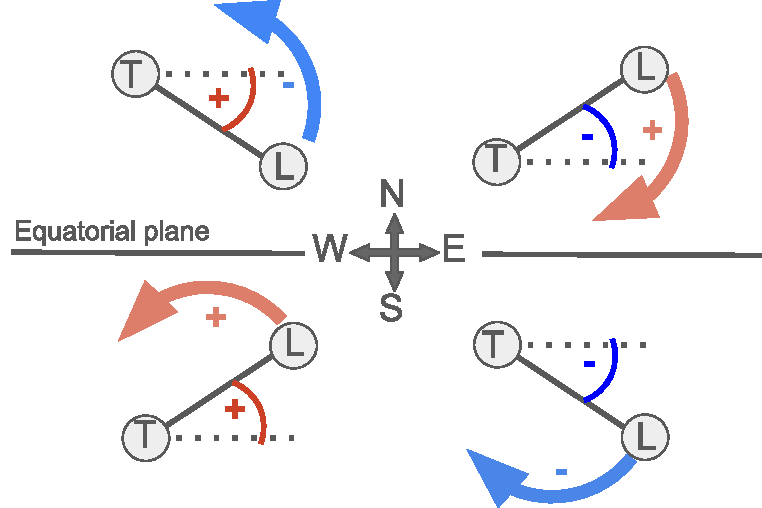
\includegraphics[width=0.9\textwidth,clip=]{./plots/diagram.pdf}}
 \caption{Diagram illustrating the sign convention used for the tilt angle ($\alpha$) and the bipole rotation ($\gamma$). The horizontal line represents the solar equator, with "T" and "L" denoting the trailing and leading polarities, respectively. Positive (negative) $\alpha$ is shown in red (blue) and corresponds to cases where the leading (trailing) polarity is closer to the equator. Positive rotation represents a shift where the leading polarity moves toward the equator, whereas negative rotation occurs when the leading polarity shifts away from the equator. }\label{fig:diag}
 \end{figure}

In general, estimating the tilt angle relies on accurately identifying the polarities of an AR. Historically, white-light images were used, where the umbra and penumbra areas of sunspots helped to pinpoint the strong flux contributions of each polarity, allowing for the identification of the centers of the leading and trailing polarities. The tilt angle was then defined by the inclination of the line connecting these two centers relative to the equatorial plane \citep[see, e.g.,][]{Baranyi16}.

However, a challenge arises when diffuse or weak magnetic flux regions, particularly in trailing polarities, fail to form clear sunspots. This issue has been resolved with the use of LOS magnetograms, which allow for clear identification of positive and negative polarities. For simple bipolar ARs, it becomes straightforward to calculate the flux-weighted centers (barycenters) of the leading and trailing polarities, enabling more precise tilt angle estimation \citep[e.g.,][]{Lopez-Fuentes00}. We will refer to this estimation of the tilt as simply $\alpha_{bar}$.
In previous studies, we compared tilt angle estimates obtained from LOS magnetograms of specific bipolar ARs with those derived from white-light images \citep{Poisson22}. Although both methods produced generally consistent results, we found that magnetic tongues significantly influence the evolution of the estimated tilt during the early phases of an AR development.

Figure~\ref{fig:diag} shows a diagram defining the sign convention used in this work for both the tilt angle ($\alpha$) and bipole rotation ($\gamma$), independently of the method used to estimate these quantities. The tilt angle is measured within a range of $-90^\circ$ to $90^\circ$. This range could pose a problem for ARs exhibiting significant rotations, as seen in some $\delta$-type sunspots. However, in our dataset of bipolar ARs, we do not find cases in which the rotation results in an East-West reversal of leading and trailing polarities. In our convention, a positive/negative tilt is assigned when the leading polarity is closer/farther to the equator in either hemisphere.
$\gamma$ reflects how the tilt evolves during a given interval of time that we set to one day. 
We define a positive/negative rotation when the leading polarity shifts toward/away the solar equator. 
The bipole rotation angle $\gamma$ tracks the changes in the AR tilt as its magnetic field evolves. A positive/negative $\gamma$ brings the leading polarity closer/farther from the equator.
These sign conventions allow for a direct comparison of tilt behavior across hemispheres.

The Bayesian method %proposed in this work offers \pc{the method is from previous works}
provides a novel measure of the emerging FR tilt.
This method describes the emergence of ARs using a magnetic FR model with a half-torus geometry, in which the twist is quantified by the number of field-line turns around the torus axis \citep[see][]{Poisson22, Poisson24}. This framework provides a simplified, large-scale description of the line-of-sight (LOS) magnetic field in bipolar ARs. While it does not include small-scale distortions due to reconnection or plasma flows during the complex emergence process, it captures the dominant magnetic structure and its temporal evolution.

To constrain the FR parameters, we generate synthetic magnetograms by computing the vertical field component onto cross-sections of the torus at different heights and comparing them with observations within a statistical Bayesian framework. The model includes four parameters describing the FR itself—minor radius ($a$), major radius ($R$), axial magnetic flux ($\Phi_A$), and twist ($N_t$)—and four positional parameters—$(x_c,y_c)$, depth $d_0$, and tilt $\alpha$. Following \citet{Poisson24}, we apply the model to time-series magnetograms, assuming that field parameters remain constant during emergence except for $a$, which evolves to account for expansion, while positional parameters vary with time. This temporal formulation improves parameter stability and ensures a coherent description of the emergence process \citep[see also][]{Poisson25}.

The presence of magnetic twist introduces at the photospheric level elongated magnetic polarities, or magnetic tongues, which evolve during the emergence. Then, the amount of twist biases the tilt estimation of the magnetic barycenter method. In contrast, using a magnetic FR model
%By design, the tilt parameter in this model 
accounts for the influence of magnetic tongues, removing their effect on the tilt, %through parametric modeling of polarity elongation along the PIL, 
then providing an estimate that aligns closer with the intrinsic inclination of the emerging FR. We will refer to this estimation of the tilt as $\alpha_{mod}$, indicating it is obtained from modeling the AR photospheric flux distribution. 



\section{Comparing Tilt Angle Estimation Methods}
\label{S-comparetilt}

\subsection{AR 9290}
\label{S-AR9290}

%% Figure AR example
%
 \begin{figure} 
 \centerline{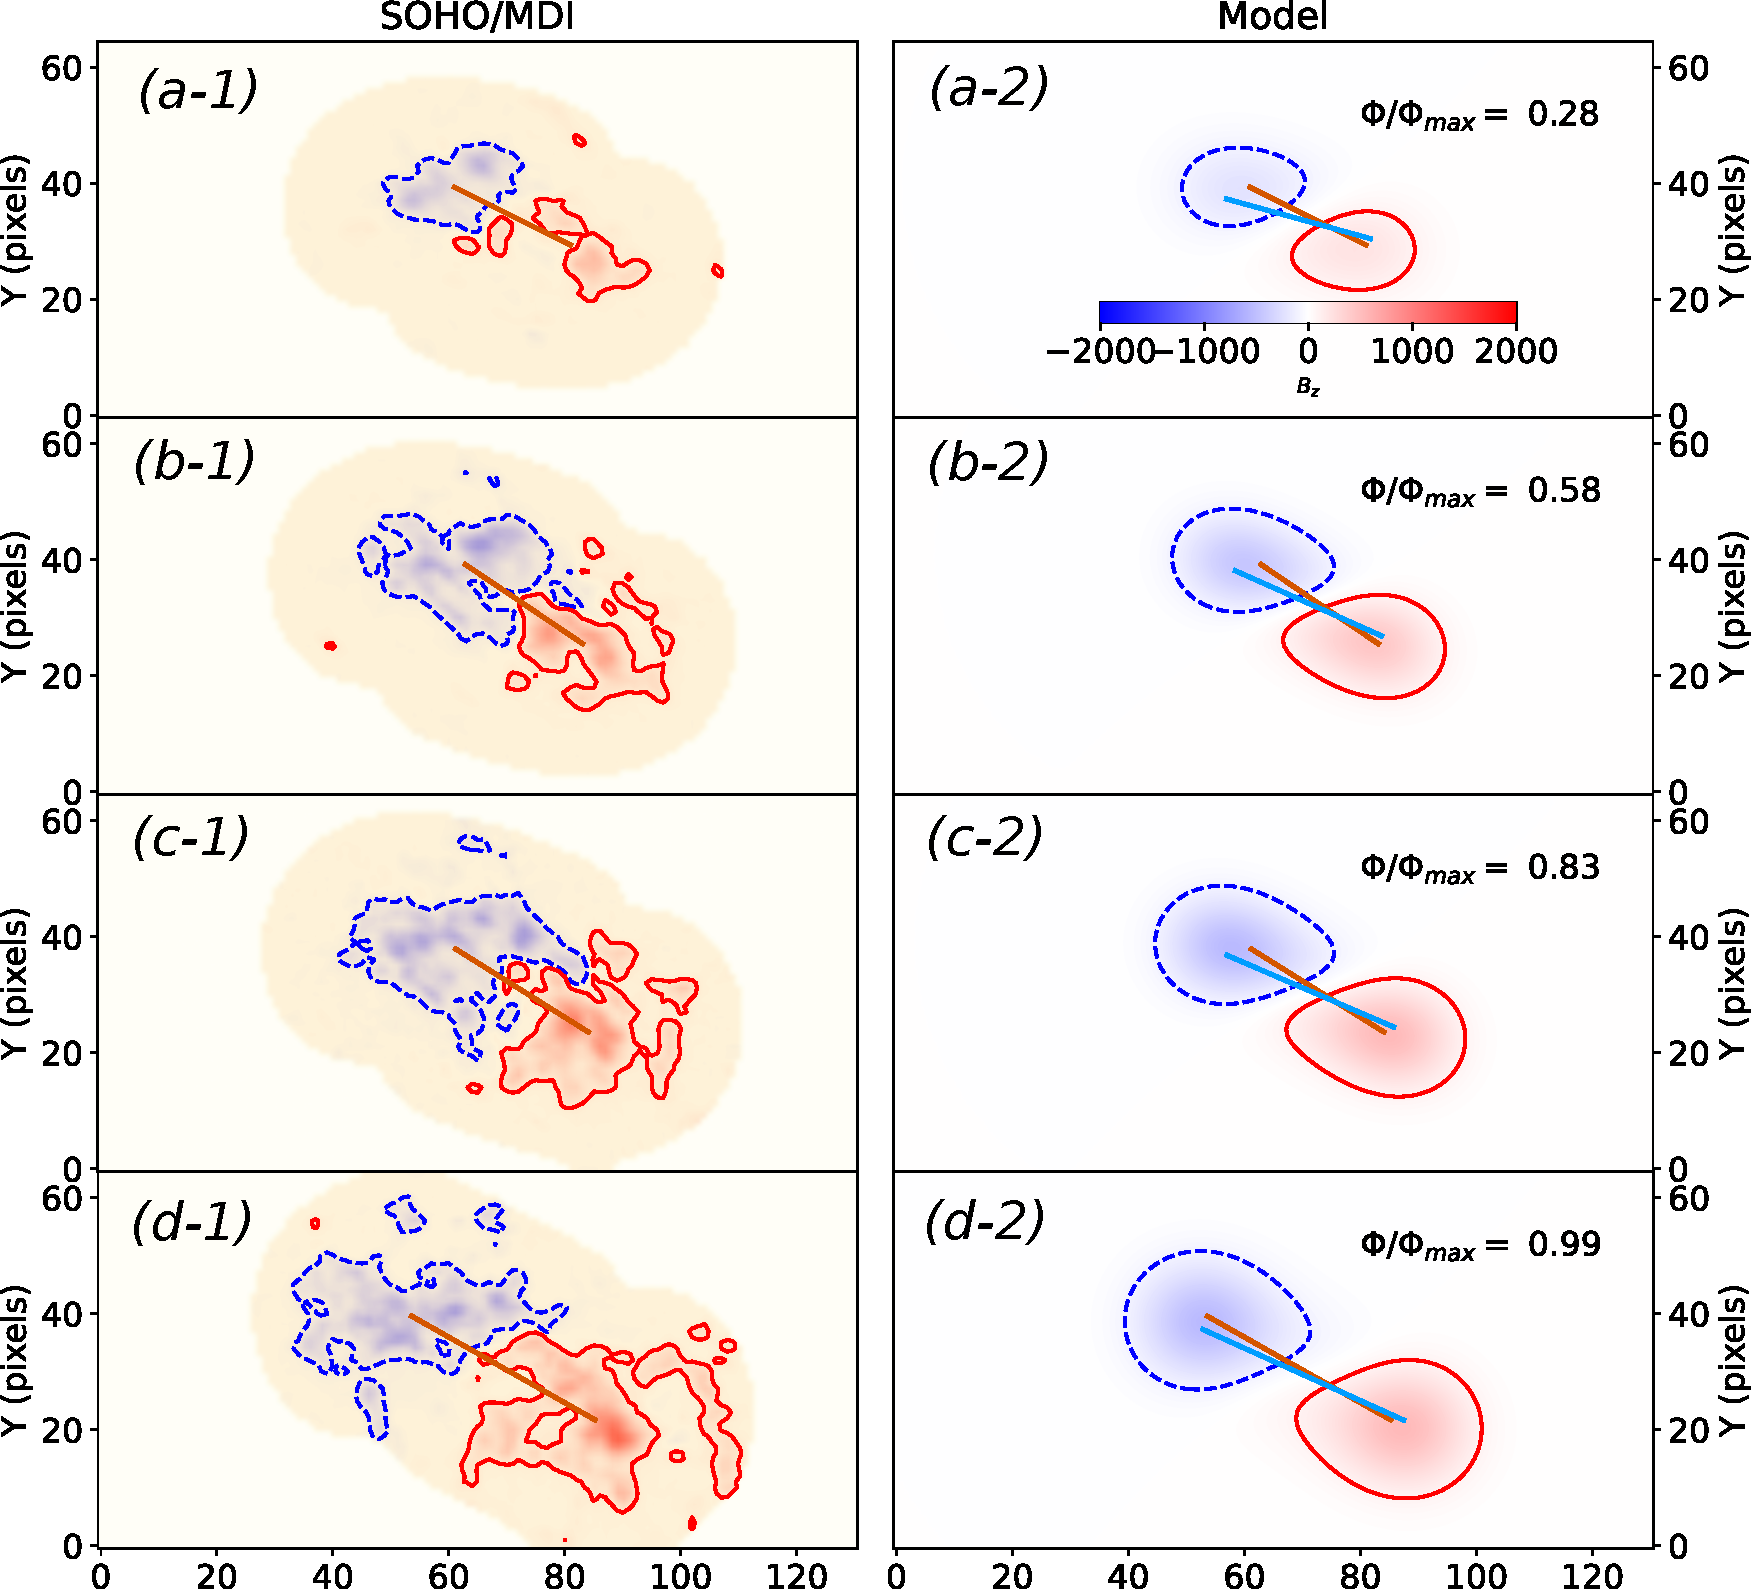
\includegraphics[width=0.9\textwidth,clip=]{./plots/9290-example.pdf}}
 \caption{Observed LOS magnetograms (left) and corresponding most probable FR models (right) at four stages of the emergence of AR 9290. Blue and red shading denote negative and positive LOS magnetic flux density, respectively. Solid red and dashed blue contours mark the $\pm100$ G levels. Orange segments connect the flux-weighted centroids of the polarities, with their orientation relative to the $x$-axis indicating the tilt derived from the magnetic barycenter method. In contrast, pale blue segments connect the modeled FR axis footpoints and provide an alternative tilt estimate obtained through the Bayesian approach. 
 }  \label{fig:9290}
 \end{figure}


Figure~\ref{fig:9290} illustrates the application of our method to AR 9290. The left panels display LOS magnetograms at representative stages of emergence while the right panels show the corresponding most probable FR models. 
The fitting masks are outlined in yellow in the left panels \citep[see][]{Poisson25}. 
The corresponding normalized magnetic flux (to the maximum flux) are indicated in the right panels. During the early phases of emergence at latitude $\sim$N$30^\circ$, the magnetic polarities appear elongated, forming magnetic tongues consistent with a negatively twisted FR. These tongues displace the flux-weighted centroids toward the polarity inversion line, leading to an apparent inclination of the bipole as measured by the barycenter method (black segments). In contrast, the modeled FR axis footpoints (green segments) provide an alternative tilt estimate that is more robust against the influence of magnetic tongues.

The temporal evolution of the tilt angle is shown in Figure~\ref{fig:evol-9290}a for both the Bayesian approach ($\alpha_\mathrm{mod}$, blue) and the barycenter method ($\alpha_\mathrm{bar}$, orange). Shaded areas indicate the $1\sigma$ uncertainties associated with each estimate. For $\alpha_\mathrm{bar}$, uncertainties were derived by averaging results obtained using four different field-strength thresholds, corresponding to all pixels, those above the median of the field-strength distribution, twice, and three times this median as a threshold for the field. 
For $\alpha_\mathrm{mod}$, the mean and standard deviation were computed from the sampled marginal posterior distribution. The time axis is normalized such that $t_\mathrm{norm}=1$ corresponds to the maximum net flux of the AR, whose evolution is shown in Figure~\ref{fig:evol-9290}b.

Both methods yield broadly consistent tilt evolution for AR 9290, though with a systematic offset of $5^\circ$–$10^\circ$ across most of the emergence. The Bayesian estimate $\alpha_\mathrm{mod}$ indicates a consistently smaller inclination than $\alpha_\mathrm{bar}$, with the maximum discrepancy occurring during the first half of emergence, when the effect of the tongues is more important. The gap narrows toward the later stages, yet does not vanish entirely, suggesting that factors beyond projection effects—such as the influence of magnetic tongues or intrinsic model assumptions—contribute to the residual differences between the two methods.


 %% Figure evol tilt 9290
%
 \begin{figure} 
 \centerline{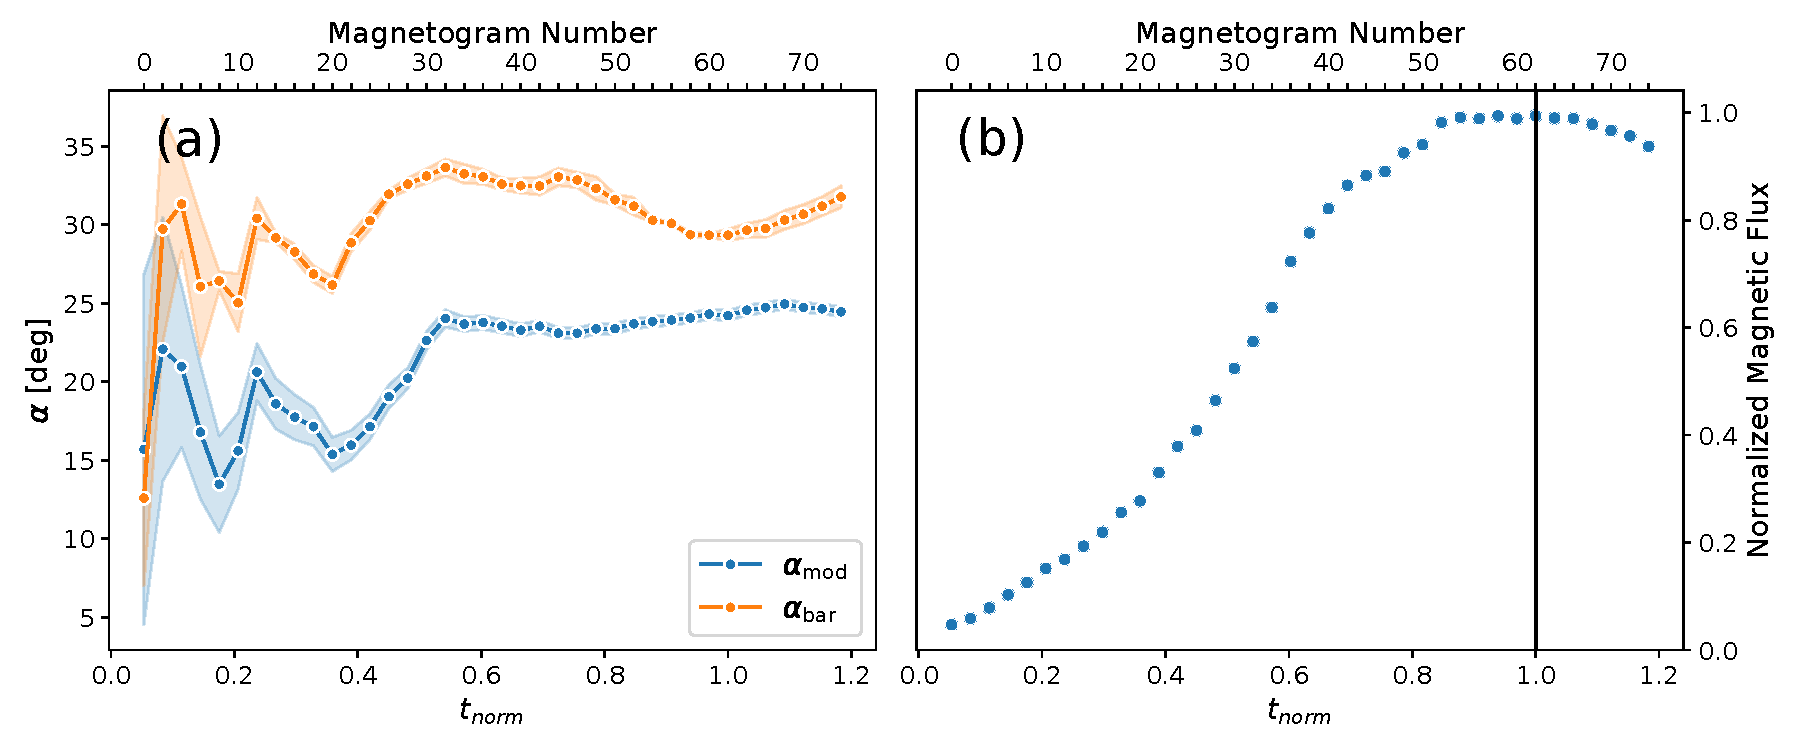
\includegraphics[width=0.99\textwidth,clip=]{./plots/9290-tilt.pdf}}
 \caption{(a) Evolution of the tilt angle, $\alpha$, of AR 9290 estimated using the Bayesian ($\alpha_{mod}$) and the barycenters methods ($\alpha_{bar}$) with blue and orange dots, respectively.  The shaded area represents the error of each estimate, as indicated by its standard deviation.  (b) Evolution of the normalized magnetic flux of AR 9290. This curve is used as a reference to determine the values of 0 and 1 for the normalized time.}\label{fig:evol-9290}
 \end{figure}

 \subsection{General Comparison}
\label{S-compareall}


In this section we compute the evolution of tilt angles for the full sample of 108 ARs using both the Bayesian FR method ($\alpha_\mathrm{mod}$) and the barycenter method ($\alpha_\mathrm{bar}$). Figure~\ref{fig:fluxes}a shows the normalized magnetic flux evolution for all ARs as a function of the normalized time $t_\mathrm{norm}$. Each dot corresponds to an estimate from a single magnetogram, while larger dots and shaded areas indicate the mean and standard deviation within different bins of $t_\mathrm{norm}$. The flux evolution curves exhibit a consistent pattern across the sample, with a rapid initial increase followed by a gradual approach to maximum flux. The dispersion in flux values is more pronounced during the early emergence stages, reflecting the variability in AR growth rates. This curve show a good correlation between the growth of $t_\mathrm{norm}$ and the AR magnetic flux suporting its use as a temporal reference for the emergence process.
The histogram in Figure~\ref{fig:fluxes}b displays the distribution of maximum magnetic flux values for the 108 ARs. The distribution is right-skewed, with a median value of $8.2 \times 10^{21}$ Mx, indicated by the red dashed vertical line. This median value is used to categorize ARs into low-flux and high-flux groups for further analysis.




 \begin{figure} 
 \centerline{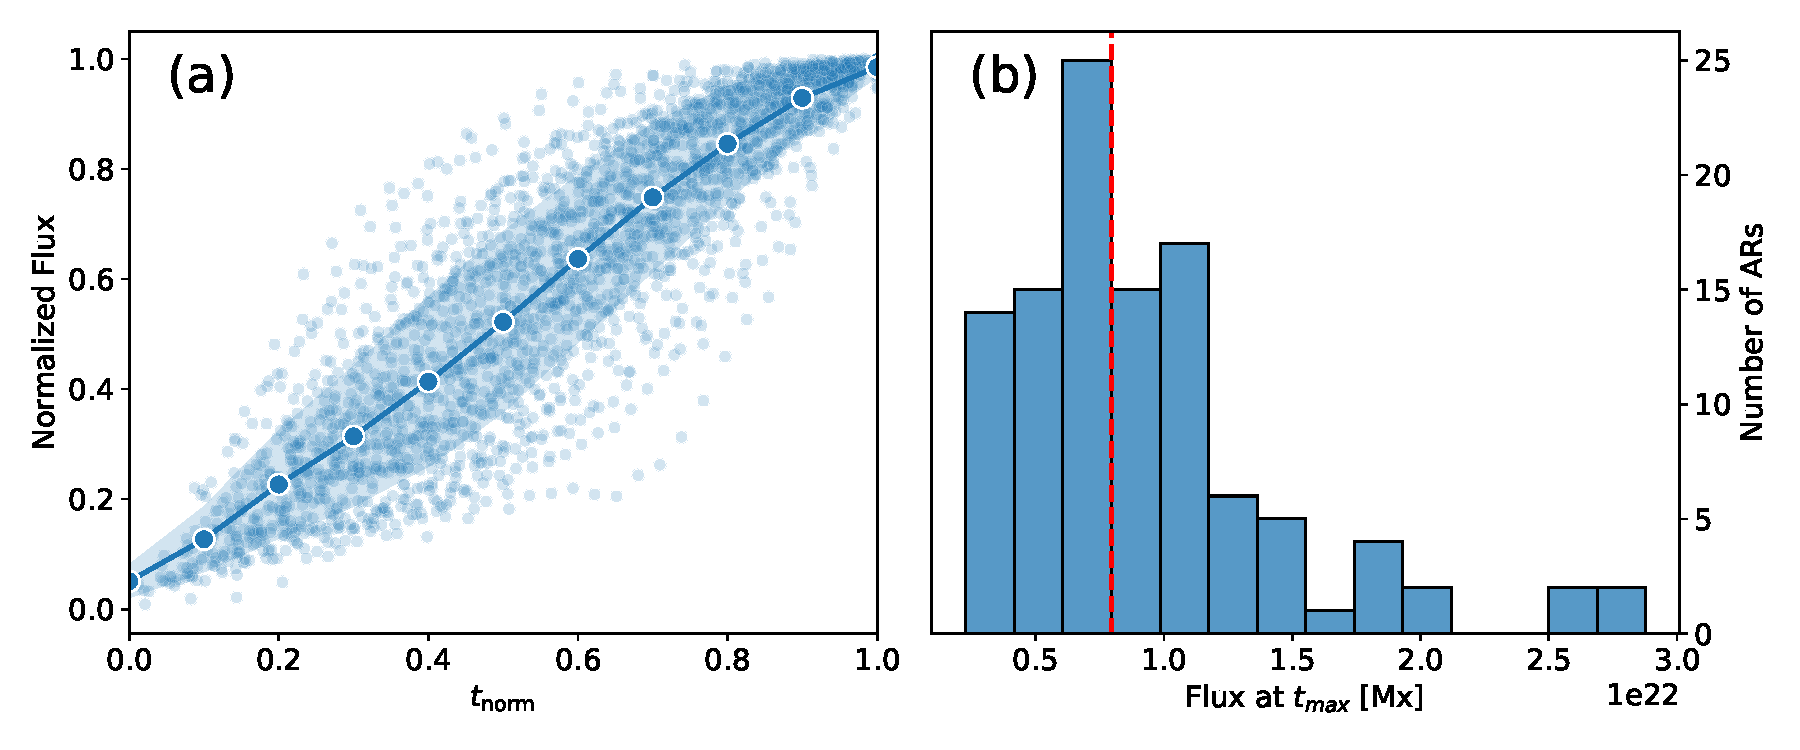
\includegraphics[width=0.99\textwidth,clip=]{./plots/flux-all.pdf}}
\caption{(a) Magnetic flux normalized to the maximum flux for 108 ARs as a function of the normalized time $t_\mathrm{norm}$. Each dot corresponds to estimates over a single magnetogram. Larger dots and shaded areas indicate the mean and standard deviation within different bins of $t_\mathrm{norm}$. (b) Histogram of the maximum magnetic flux of the ARs. Red-dashed vertical line indicates the median of the distribution showing the samples used to group low and high flux ARs}
\label{fig:fluxes}
 \end{figure}

 We assess the correlation between the two tilt estimates for the 108 ARs by comparing $\alpha_\mathrm{mod}$ with $\alpha_\mathrm{bar}$ (Figure~\ref{fig:alpha-alpha}a). Each point corresponds to the mean tilt value of a given AR within one of eleven bins defined along the normalized time axis ($0 \leq t_\mathrm{norm} \leq 1$). This procedure yields a total of 1111 points, fewer than the 1188 possible, since some ARs lack measurements close to the first bin near $t_\mathrm{norm}=0$. A linear least-squares fit to the scatter plot gives a slope of $0.57$ and a Pearson correlation coefficient of $0.63$, indicating a moderate correlation between the two methods. On average, the Bayesian estimates yield systematically smaller tilt angles than the barycenter method. High-flux and low-flux ARs, represented by orange and green lines respectively, exhibit similar trends, with slopes of $0.50$ and $0.64$ and correlation coefficients of $0.61$ and $0.66$, respectively. This consistency suggests that the systematic differences between the two methods are not strongly dependent on the AR magnetic flux.

The comparison of tilt signs further reveals that $\sim 63\%$ of the values correspond to positive tilts for both methods, i.e., with the leading polarity closer to the equator.
In contrast, $\sim22\%$ of the cases show negative tilts in both estimates. Discrepancies of tilt sign between the two approaches arise in the remaining fraction of cases: about $10\%$ are positive in $\alpha_\mathrm{mod}$ but negative in $\alpha_\mathrm{bar}$, while $\sim6\%$ show the opposite behavior. These differences highlight the sensitivity of the tilt sign determination to the method employed, particularly in bipoles which are closely oriented towards the EW direction.

Figure~\ref{fig:alpha-alpha}b shows the histograms of the mean tilt values per AR per bin along $t_\mathrm{norm}$. The two methods yield very similar distributions, both in terms of mean values and dispersion, with $\alpha_\mathrm{mod}$ shown in blue and $\alpha_\mathrm{bar}$ in orange. This indicates that, despite the systematic differences seen in the direct comparison, both estimations capture a consistent range of tilt angles within our sample of ARs.

 \begin{figure} 
 \centerline{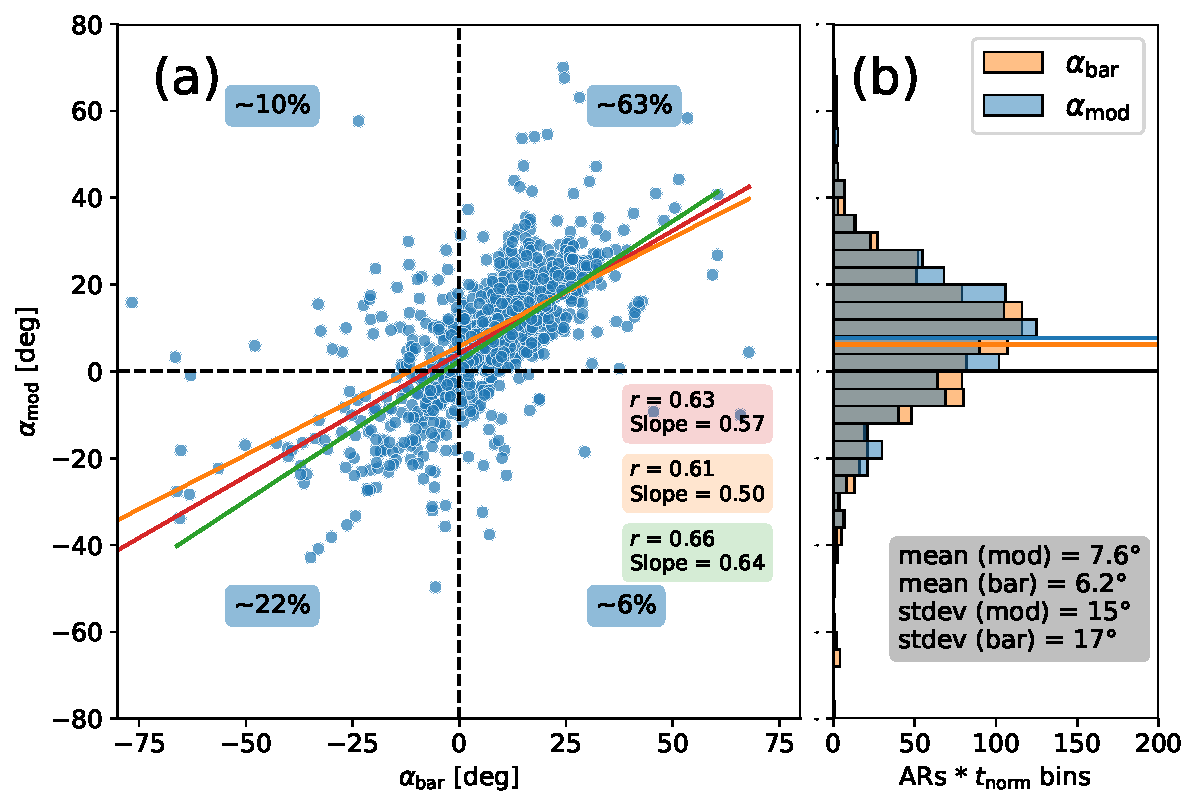
\includegraphics[width=0.99\textwidth,clip=]{./plots/alpha-alpha.pdf}}
\caption{(a) Comparison of tilt angles estimated with the Bayesian FR method ($\alpha_\mathrm{mod}$) and the barycenter method ($\alpha_\mathrm{bar}$) for 108 ARs. Each point represents the mean tilt within a $t_\mathrm{norm}$ bin. The red, orange, and green lines show the linear least-squares fit of the full sample, the high-flux sample, and the low-flux sample, respectively. (b) Histogram of tilt angle distributions for both methods, with $\alpha_\mathrm{mod}$ in blue and $\alpha_\mathrm{bar}$ in orange.}
\label{fig:alpha-alpha}
 \end{figure}

   \begin{figure} 
 \centerline{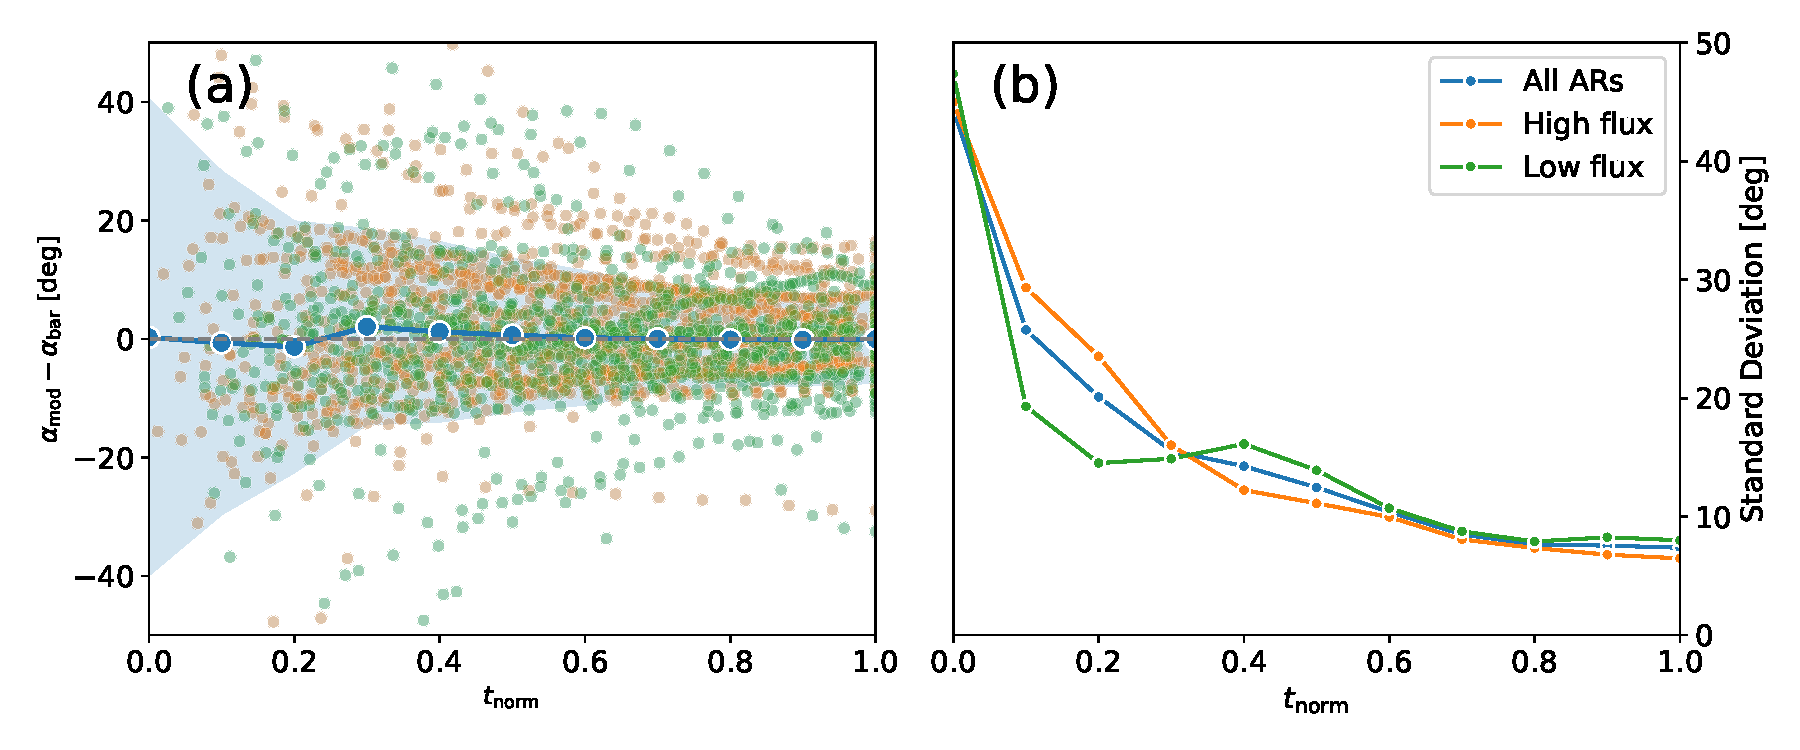
\includegraphics[width=0.99\textwidth,clip=]{./plots/alpha-err.pdf}}
 \caption{(a) Evolution of the difference between Bayesian FR and barycenter tilt estimates ($\alpha_\mathrm{mod}-\alpha_\mathrm{bar}$) for all analyzed magnetograms of 108 ARs. Blue dots indicate the median value within each $t_\mathrm{norm}$ bin, and the shaded area represents the 1-$\sigma$ standard deviation. Green and orange dots corresponds to the difference for ARs with lower and higher flux respectively. (b) Evolution of the 1-$\sigma$ standard deviation of the difference between tilt estimations for the same groups.}\label{fig:diff-alpha}
 \end{figure}

We compute the difference between the two methods as $\alpha_\mathrm{mod} - \alpha_\mathrm{bar}$ and analyze how it evolves during the emergence of 108 ARs. Figure~\ref{fig:diff-alpha}a shows this difference as a function of $t_\mathrm{norm}$, which provides a common temporal reference for the different {ARs}. Solid blue dots with connecting lines correspond to the median values {at each temporal bin, and} the shaded areas indicate the corresponding standard deviation. The green and orange dots represent the differences for low-flux and high-flux ARs, respectively. Across the entire sample, the median difference remains close to zero throughout the emergence process, indicating no significant systematic bias between the two methods on average. However, the standard deviation of the differences, shown in Figure~\ref{fig:diff-alpha}b, reveals a clear trend: it decreases from approximately $40^\circ$ at $t_\mathrm{norm} = 0$ to about $8^\circ$ at $t_\mathrm{norm} = 1$. This indicates that the two methods converge toward similar tilt estimates as the ARs approach their maximum flux.


The largest difference between $\alpha_\mathrm{mod}$ and $\alpha_\mathrm{bar}$ during the early stages of emergence is expected due to the influence of magnetic tongues, which decrease as the tongues retract toward the end of emergence. The distribution of differences becomes close to normal for $t_\mathrm{norm} \ge 0.5$, symmetrically distributed around a mean of zero. These distributions with decreasing standard deviations suggest that our sample includes a wide variety of effects that bias the barycenter-based estimation of the tilt. In particular, the normal distribution indicates that the emerging FRs likely span a broad range of twist values, producing tongues of different strengths and, consequently, varying projection effects on $\alpha_\mathrm{bar}$. 


Figure~\ref{fig:alpha-gamma}a shows the temporal evolution of the tilt angle, $\alpha$, as a function of $t_\mathrm{norm}$ for the full sample of 108 ARs. The blue and orange curves correspond to values derived from the tilt angles obtained with the model ($\alpha_\mathrm{mod}$) and with the magnetic barycenters ($\alpha_\mathrm{bar}$), respectively. Both methods reveal a broadly similar trend despite case by case differences presented in Figure~\ref{fig:diff-alpha}. Median values represented by solid dots connected with lines mantain stable between $\sim6^\circ$ and $\sim10^\circ$ throughout the emergence process. The broad dispersion of points reflects the large variability in the tilt angles across different ARs, including different fluxes and latitudes of emergence.



   \begin{figure} 
 \centerline{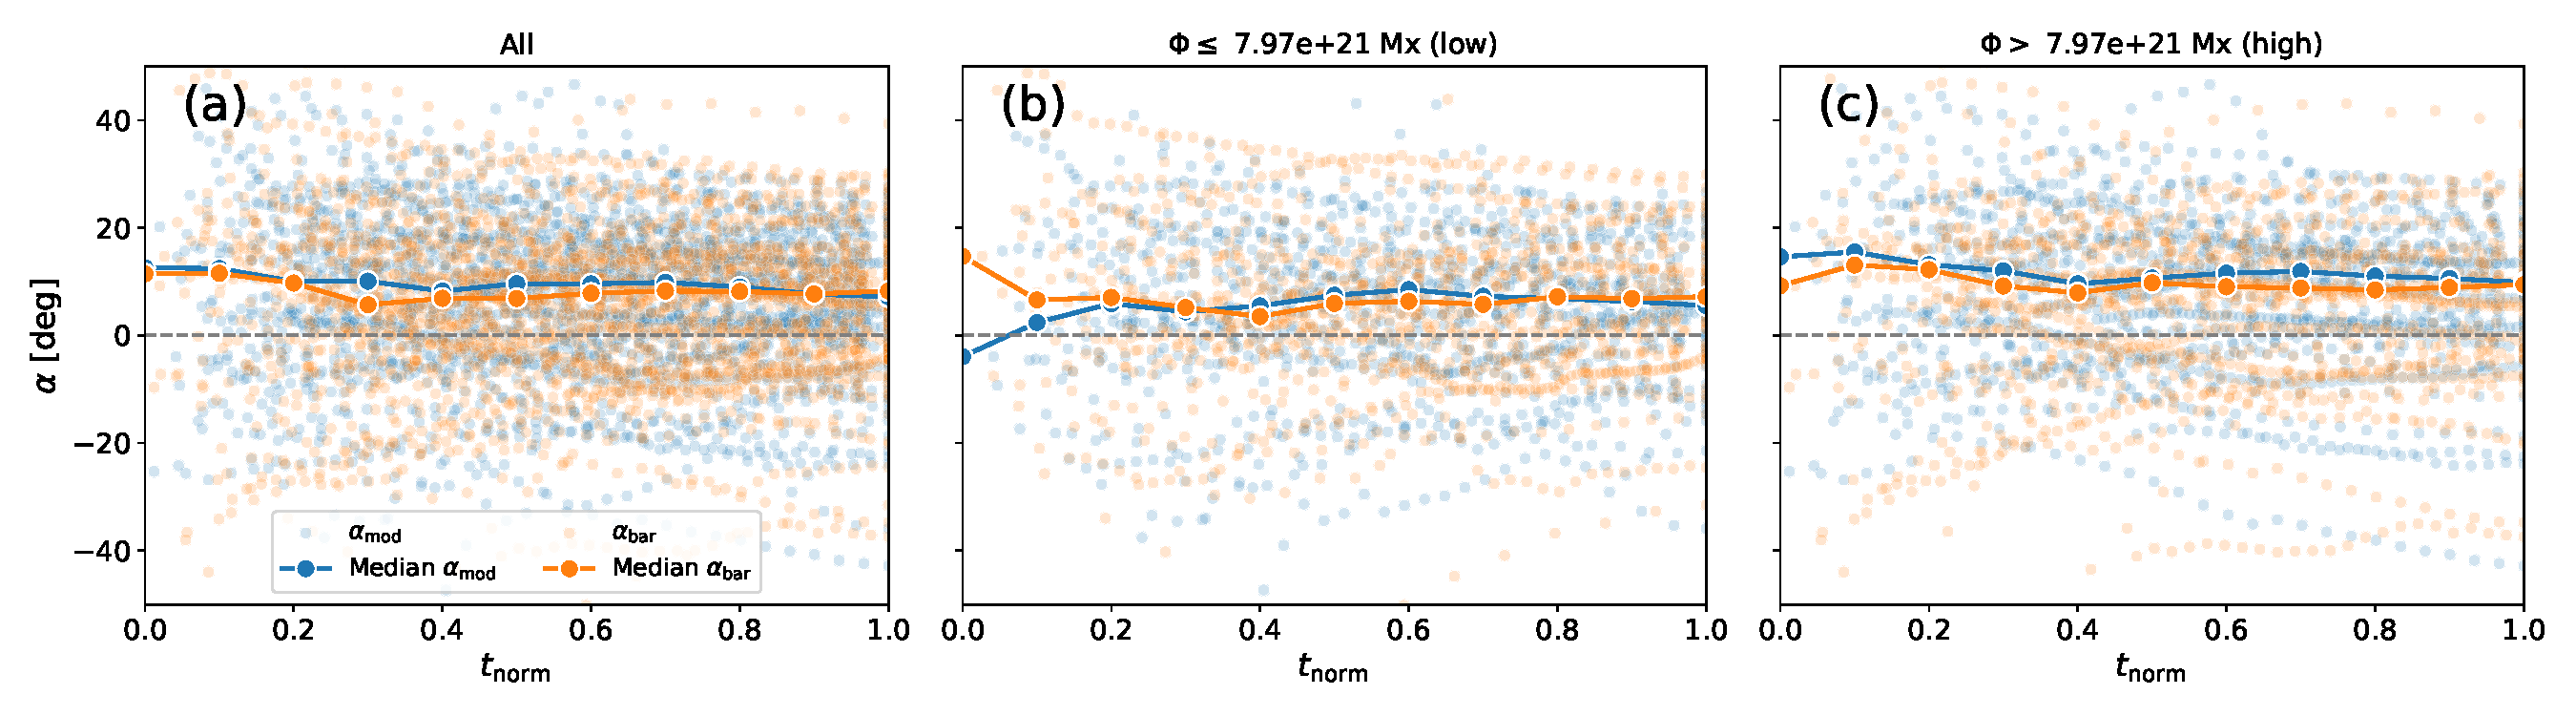
\includegraphics[width=0.99\textwidth,clip=]{./plots/alpha-vs-t_norm.pdf}}
  \centerline{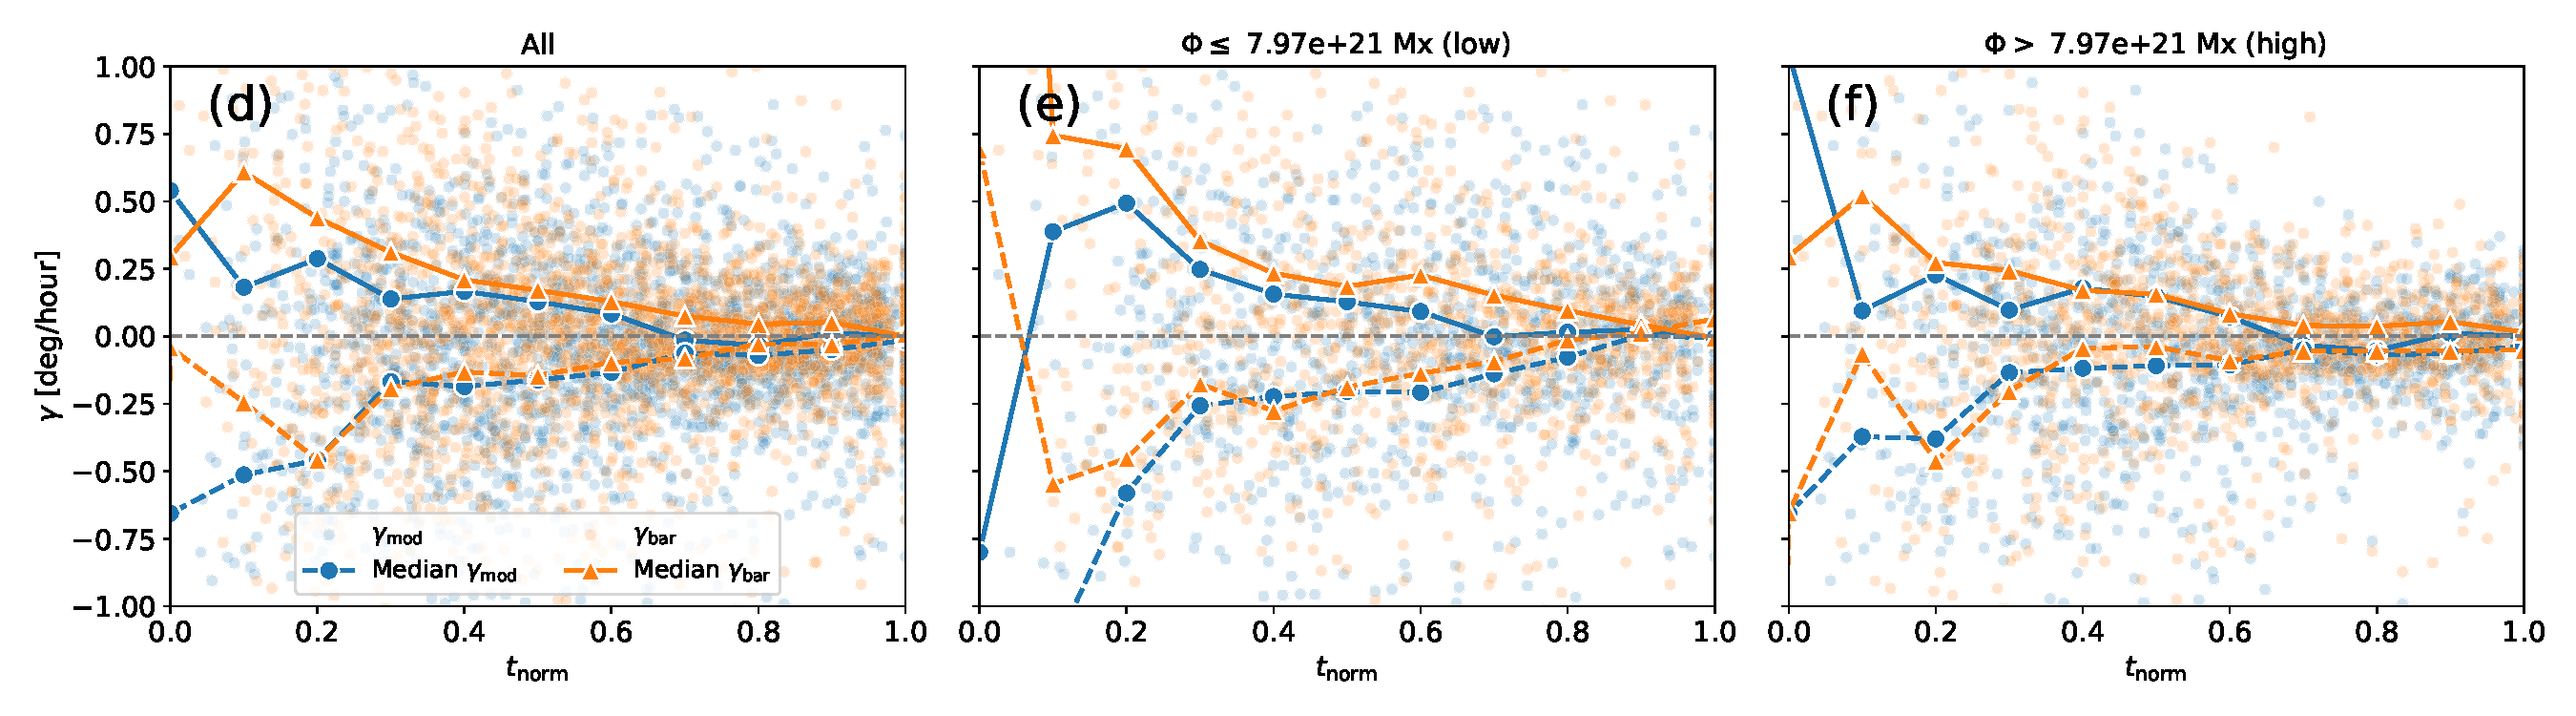
\includegraphics[width=0.99\textwidth,clip=]{./plots/gamma-vs-t_norm.pdf}}
 \caption{Top row: Evolution of the tilt angle for 108 ARs. Dots indicate the estimation of $\alpha$ obtained with the Bayesian method (blue) and the barycenter method (orange). Solid dots indicate the median value within each $t_\mathrm{norm}$ bin for each estimate. We group the sample using all 108 ARs (a), those with low magnetic flux (b), and those with higher flux (c). Bottom row: Evolution of the angular rotation rate $\gamma$ for all 108 ARs (d), low flux (e), and high flux ARs (f). Solid (dashed) lines join median values within $t_\mathrm{norm}$ bins for ARs in which total accumylated rotation is positive (negative).
 } \label{fig:alpha-gamma}
 \end{figure}





Figure~\ref{fig:alpha-gamma}b and c display the evolution of $\alpha$ for the low-flux and high-flux sub-samples, respectively. For both estimation methods the high-flux ARs present systematically larger tilt angles than the low-flux ARs, an effect that is most noticeable during the early stages of emergence. The shift in the median tilt between the two groups is driven largely by a reduction in the number of negative-tilt cases in the high-flux sample (fewer occurrences where the leading polarity is displaced away from the equator). This finding suggests that stronger, high-flux regions are less prone to the tongue-induced or convective biases that inflate the occurrence of negative tilts at low flux. This effect is more clearly captured by the Bayesian estimate $\alpha_\mathrm{mod}$, which yields a cleaner signal with reduced scatter.

We compute the rotation rate of the bipole $\gamma$ as a function of $t_{\mathrm{norm}}$ in Figure~\ref{fig:alpha-gamma}d. We separated ARs with a positive (solid lines) and negative (dashed lines) total accumulated rotation. Blue dots and orange triangles indicate the median of $\gamma$ within temporal bins. Both estimates present similar trends in which rotations are stronger at early phases of the emergence and tilts tend to stabilize by the time of the maximum flux. Panels (e) and (f) show same trend for $\gamma$ for the low-flux and high-flux sub-samples. Comparing these samples we find that low-flux ARs presents stronger mean rotations along the emergence by a factor 2 than the high-flux ARs.


The larger dispersion of $\gamma_{\mathrm{bar}}$ during early emergence (compared to $\gamma_{\mathrm{mod}}$) indicates that barycenter-based rotation estimates are more affected by transient effects such as magnetic tongues and small-scale flux rearrangements, while the Bayesian FR estimate provides a cleaner, more stable measure of the intrinsic bipole rotation. The decreasing trend observe for both estimates is more likely associated to the emergence process in which convective buffeting over the FR is less effective as the AR flux increases and polarities apart from each other.


    \begin{figure} 
      \centerline{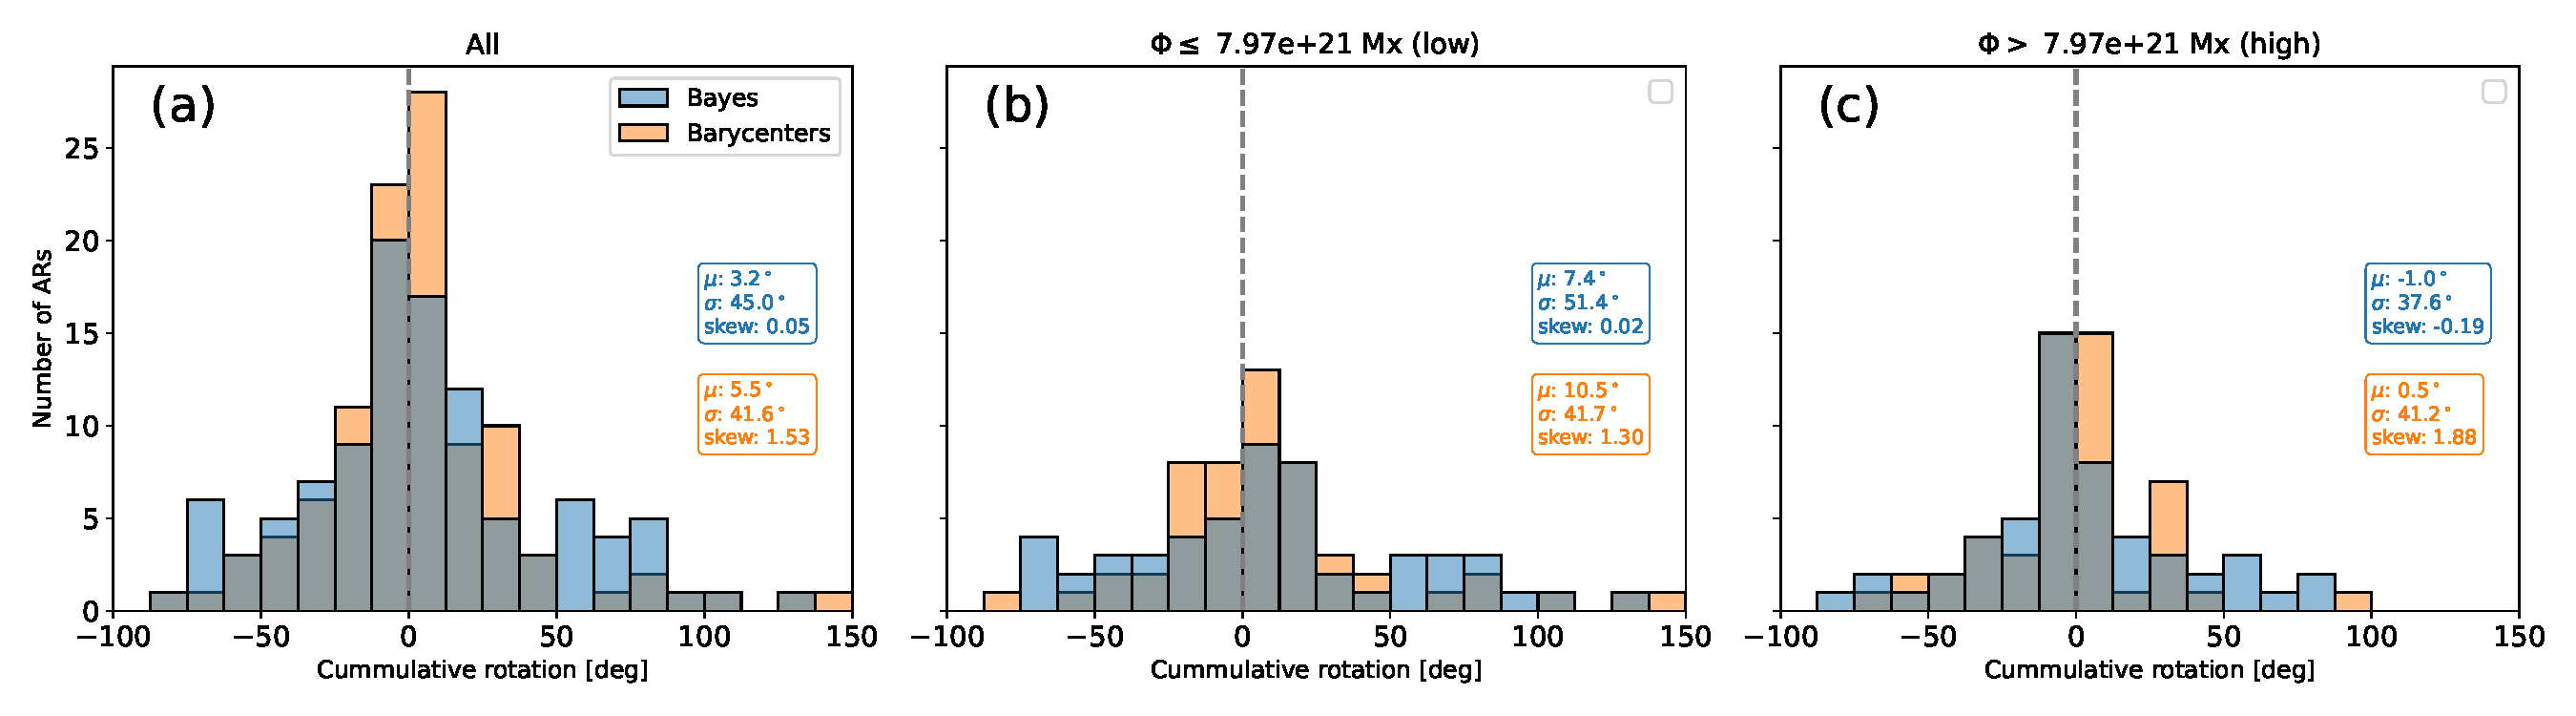
\includegraphics[width=0.99\textwidth,clip=]{./plots/hist_cumrot.pdf}}
      \caption{Distribution of the cumulative rotation during AR emergence. Blue and orange histograms show cumulative rotations obtained with the Bayesian method and the barycenter method, respectively. Panels correspond to (a) the full sample of 108 ARs, (b) the low–flux subsample, and (c) the high–flux subsample.}
      \label{fig:cum-gamma}
    \end{figure} 

    Figure~\ref{fig:cum-gamma} shows the distribution of the total accumulated rotation,
    computed as $\sum_{t=0}^{1}\gamma\,\Delta t$, for (a) the full sample of 108 ARs, (b) the low–flux subsample, and (c) the high–flux subsample. In each panel blue and orange histograms correspond to the Bayesian and barycenter estimates, respectively. Both methods yield similar central values and overall dispersions, indicating comparable rotation magnitudes on average. However, the Bayesian-derived distributions are generally more symmetric and closer to a normal shape, while the barycenter-derived distributions display larger skewness. This reduced asymmetry suggests the Bayesian method produces more robust cumulative-rotation estimates by mitigating biases from magnetic tongues and short-term flux rearrangements; the near-symmetric Bayesian distributions are consistent with convective buffeting acting predominantly as a stochastic driver of bipole rotation. \mpc{Still effect is small over few cases and both methods suggest that convective buffeting is the main contribution to AR rotations.}  

  
\section{Latitudinal dependance of the Tilt Angle} %Methods %%%%%%%%%%%%%%
  \label{S-latitude}


  



   \begin{figure} 
 \centerline{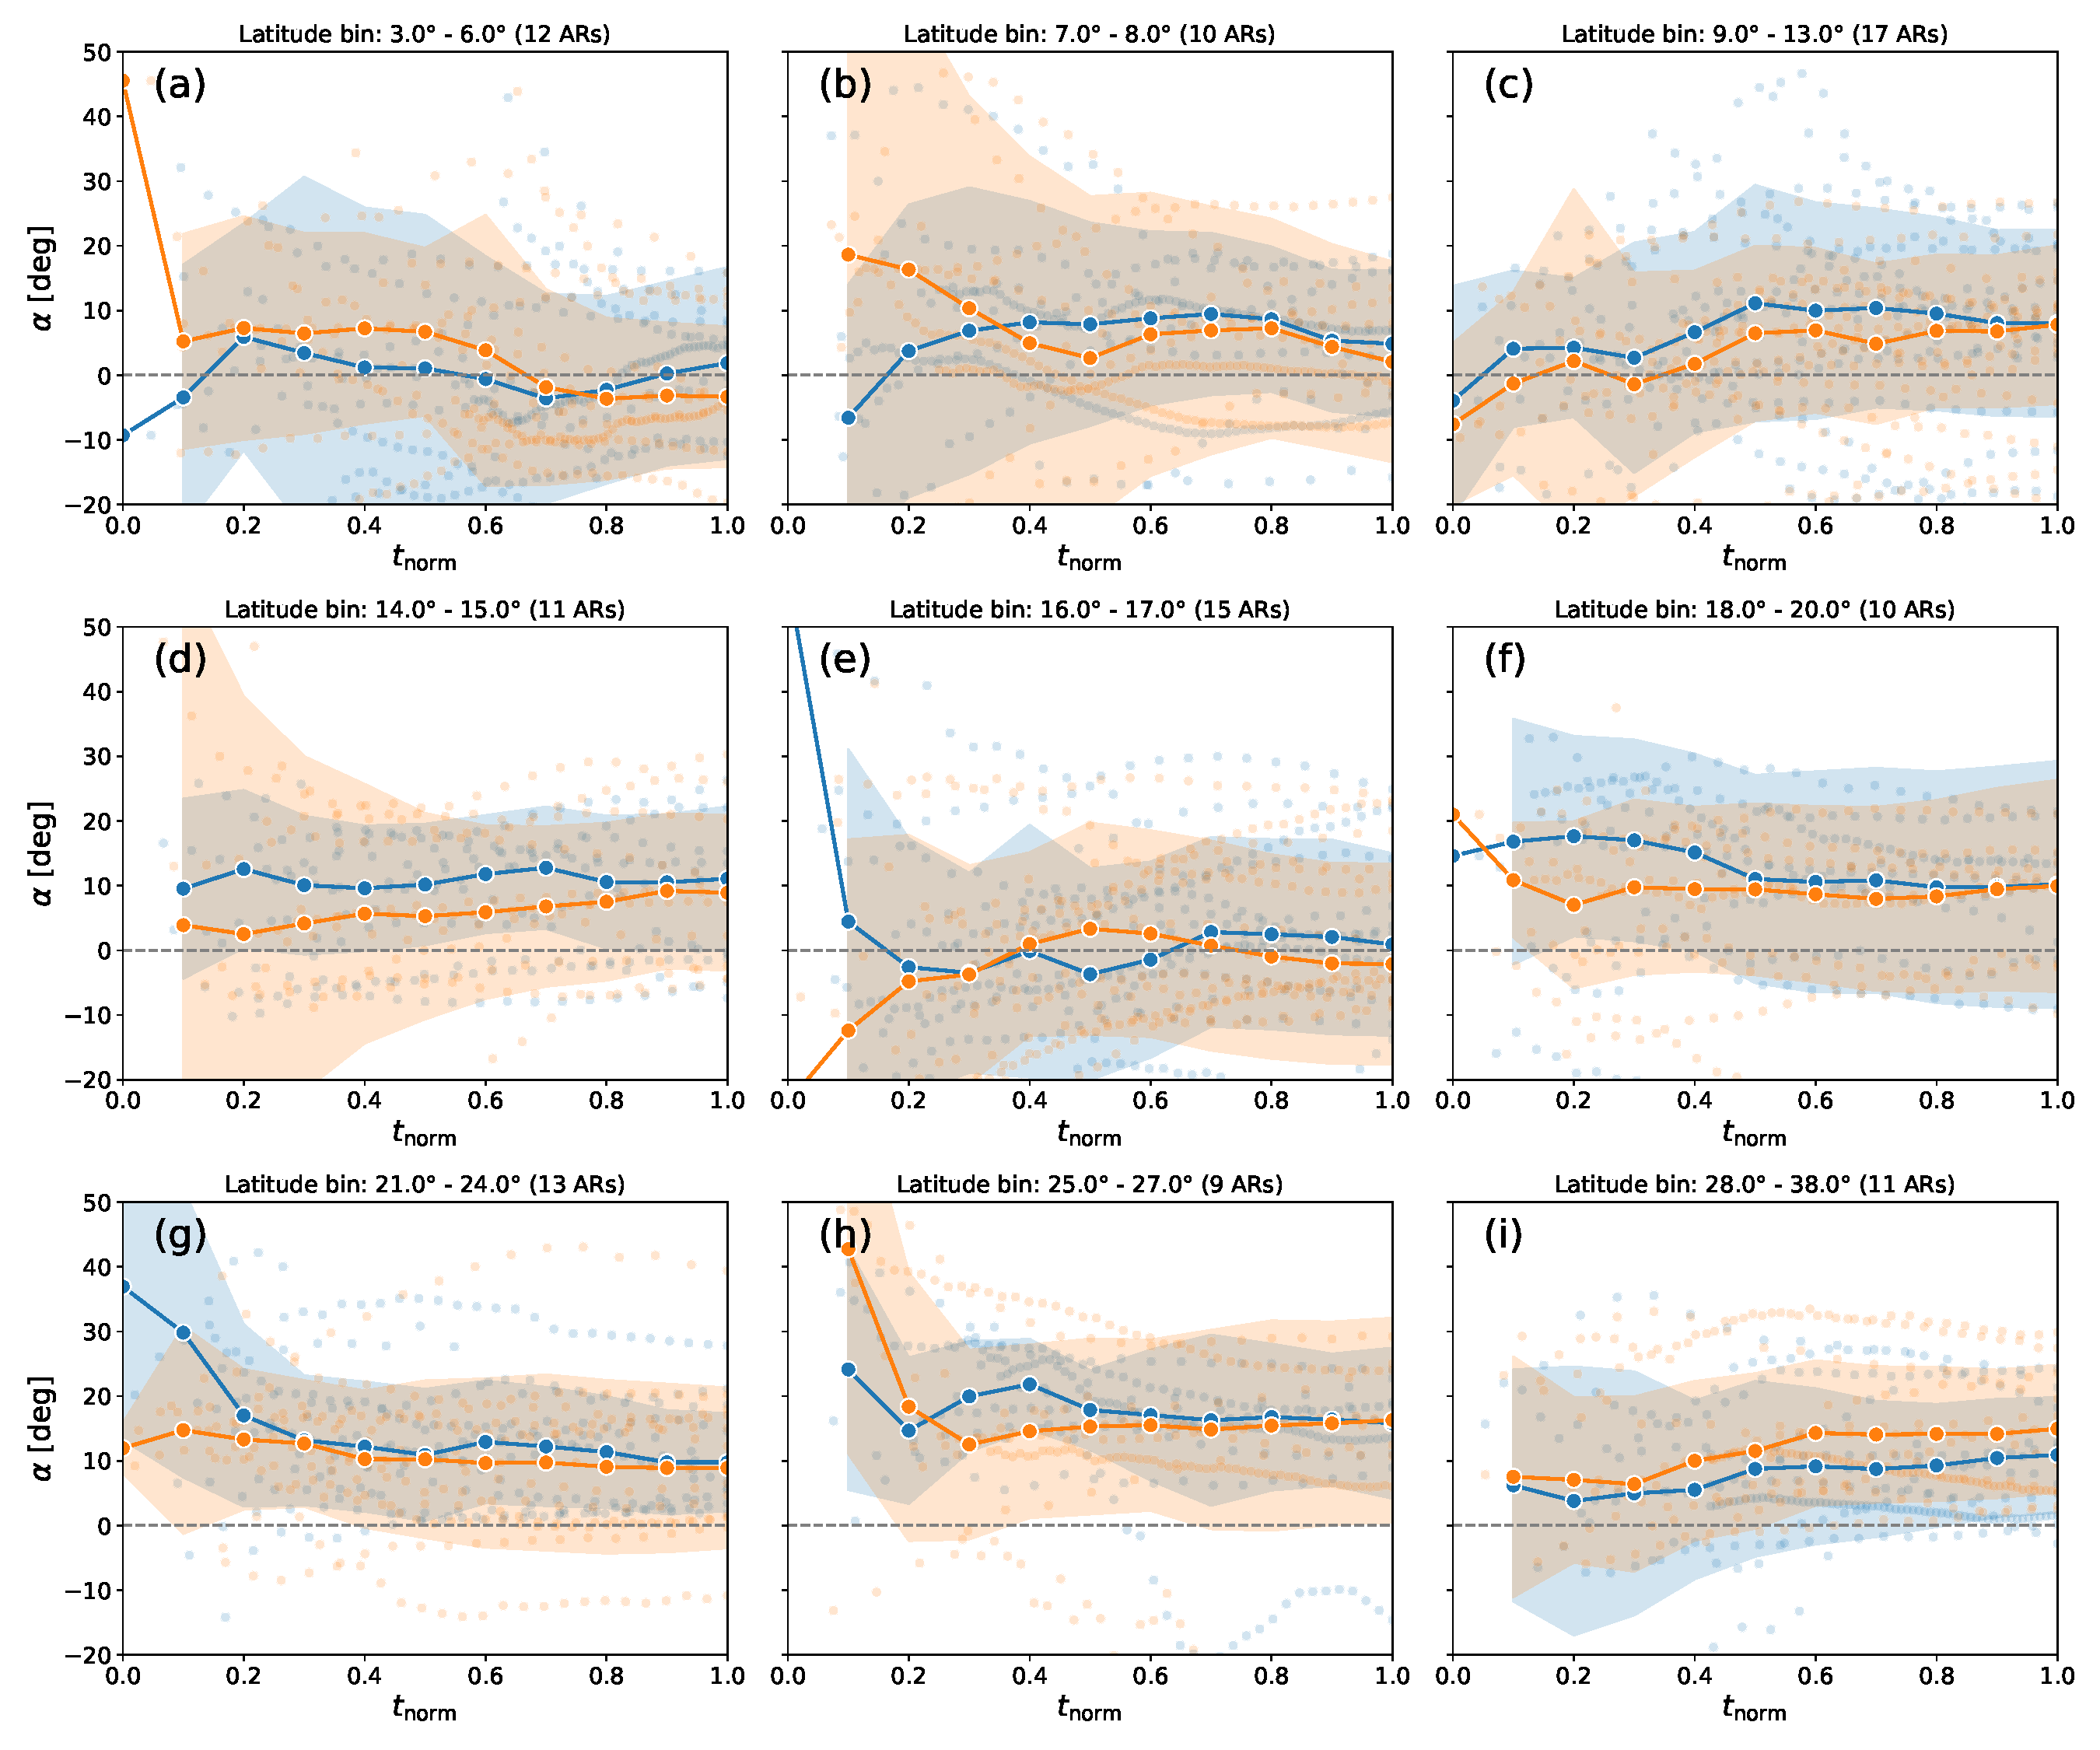
\includegraphics[width=0.99\textwidth,clip=]{./plots/alpha-vs-t_norm-by-lat.pdf}}
 \caption{Evolution of $\alpha$ as a function of the normalized time $t_\mathrm{norm}$ for different latitudinal bins. Each panel corresponds to a specific latitude bin, with solid lines representing the median $\alpha$ values and shaded areas indicating the standard deviation. Scatter points show individual data points.} \label{fig:alpha-lat}
 \end{figure}


   \begin{figure} 
 \centerline{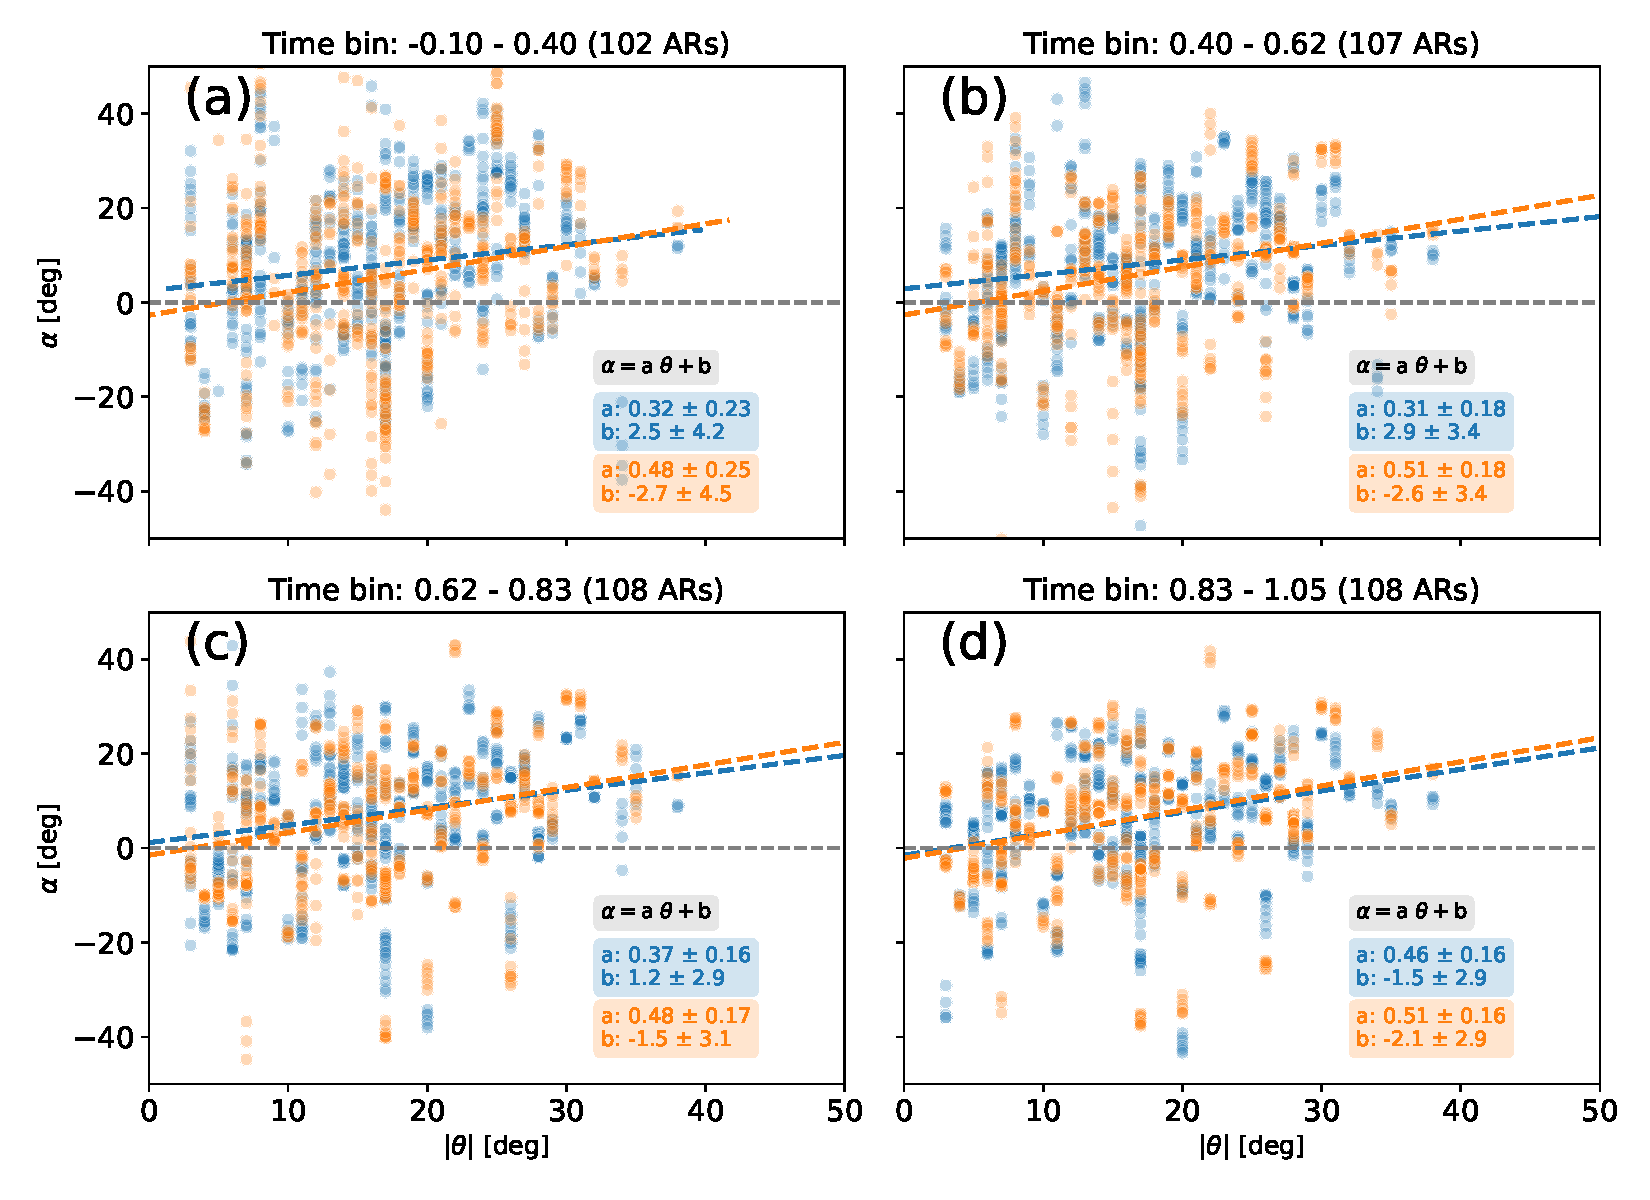
\includegraphics[width=0.99\textwidth,clip=]{./plots/alpha-vs-lat-by-tnorm.pdf}}
 \caption{Mean tilt as a function of latitude for different normalized time bins. Each panel corresponds to a specific normalized time bin, with blue (orange) dots representing $\alpha_\mathrm{mod}$ ($\alpha_\mathrm{bar}$) individual data points. The dashed lines indicate the linear least-squares fits for both methods.} \label{fig:alpha-lat}
 \end{figure}

\begin{table}[ht]
\centering
\caption{RMS error and Pearson correlation (rho) by time bin.}
\label{tab:timebins}
\begin{tabular}{lcccc}
\hline
Time bin & RSME $\alpha$ (deg) & $\rho_{\alpha}$ & RSME $\alpha_{\mathrm{bar}}$ (deg) & $\rho_{\alpha_{\mathrm{bar}}}$ \\
\hline
-0.10 -- 0.40 & 17.67 & 0.1397 & 18.97 & 0.1926 \\
0.40 -- 0.62  & 14.93 & 0.1598 & 14.75 & 0.2621 \\
0.62 -- 0.83  & 13.05 & 0.2206 & 13.84 & 0.2656 \\
0.83 -- 1.05  & 12.72 & 0.2742 & 13.10 & 0.2971 \\
\hline
\end{tabular}
\end{table}


   \begin{figure} 
 \centerline{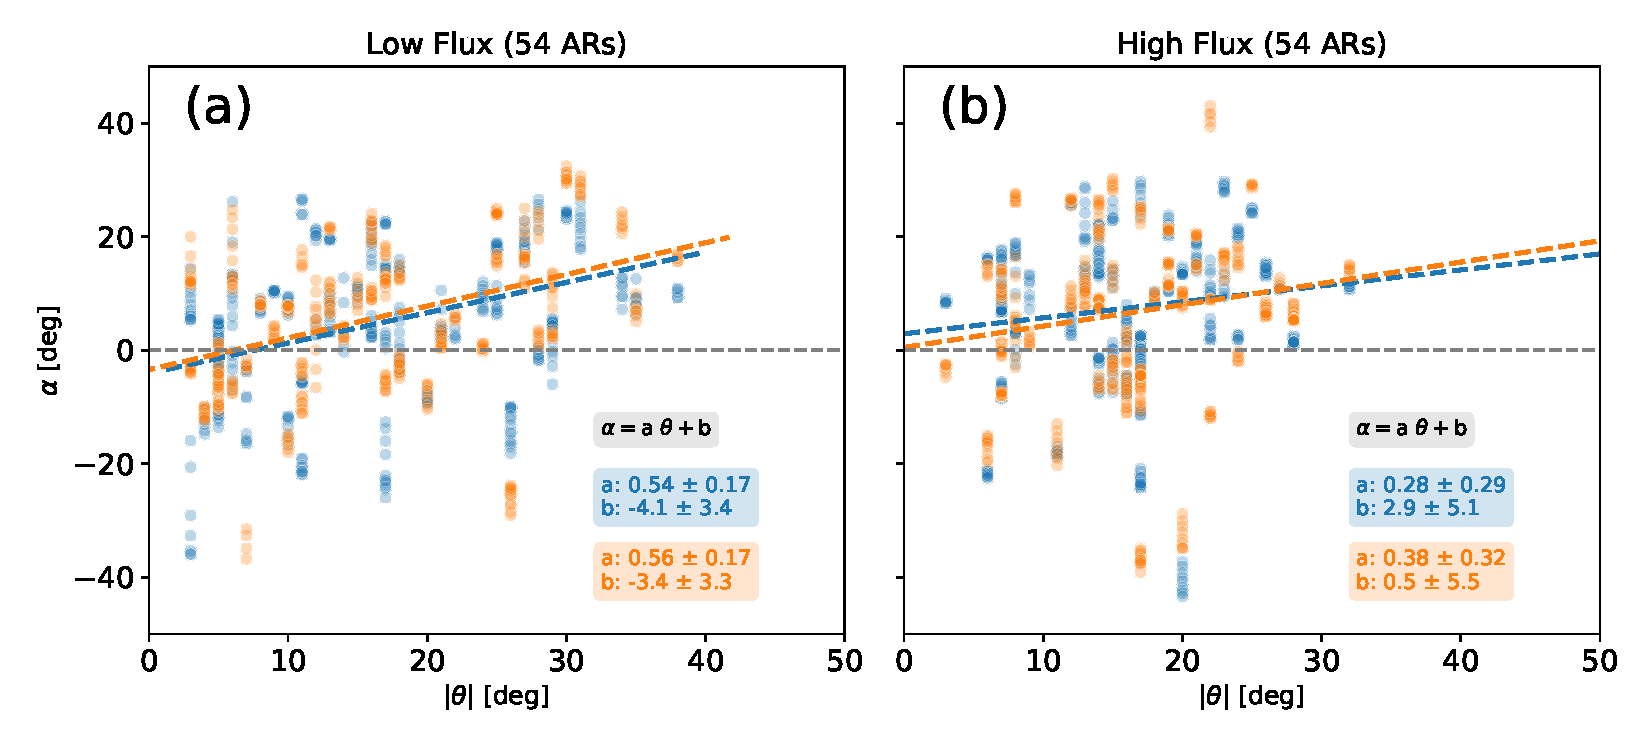
\includegraphics[width=0.99\textwidth,clip=]{./plots/alpha-vs-lat-by-flux.pdf}}
 \caption{Mean tilt as a function of latitude for low (a) and high (b) flux ARs. On each panel the blue (orange) dots represents $\alpha_\mathrm{mod}$ ($\alpha_\mathrm{bar}$) individual data points. The dashed lines indicate the linear least-squares fits for both methods.} \label{fig:alpha-lat-by-flux}
 \end{figure}

\begin{table}[ht]
\centering
\caption{RMS error and Pearson correlation by flux group.}
\label{tab:fluxgroups}
\begin{tabular}{lcccc}
\hline
Group & RMSE $\alpha$ (deg) & $\rho_{\alpha}$ & RMSE $\alpha_{\mathrm{bar}}$ (deg) & $\rho_{\alpha_{\mathrm{bar}}}$ \\
\hline
Low Flux  & 11.68 & 0.391216 & 11.55 & 0.409670 \\
High Flux & 13.48 & 0.131941 & 14.59 & 0.161803 \\
\hline
\end{tabular}
\end{table}
  
 
 
%% Figure tilts
%
% \begin{figure} 
% \centerline{\includegraphics[width=0.95\textwidth,clip=]{./plots/alphas.pdf}}
% \caption{Mean daily tilt obtained for the 126 ARs. The histograms show the mean tilt values obtained using the Bayesian FR method (blue) and with the magnetic barycenters (orange). When the two distributions superpose the bars have a brown color. Panels correspond to the day of emergence of ARs: first, second, and third day of the emergence are grouped in panels (a), (b), and (c), respectively. The histogram corresponding to days 4 and 5 is plotted in panel (d). The black-dashed vertical line indicates the value of $\alpha = 0$. The colored vertical lines show the mean \pc{better to show the median (more stable with low number of cases and to outsiders)} of each distribution. We include an inset indicating the number of positive and negative tilt values on each distribution.  \pc{This inset can be both more compact and making easier the comparison. See comment on the pdf but may be better in rows: one row for $\alpha >0$ and one row for $\alpha <0$ (so easier to compare numbers). Also I would add median, standard deviation and skewness of both distributions (one row for median, one row for standard deviation, one row for skewness). Use a classical symbol for each.  2 significant digits could be sufficient.}  }
% \label{fig:alphas}
% \end{figure}


  \subsection{Filtering effect of turbulent buffeting}
%  \subsection{Tilt from Bayesian Models}
      \label{S-filter}

\mpc{Reducing outliers assuming a latitudinal dependence $\propto \sin (\theta)$}


\subsection{Comparing Joy's Law}
\label{S-Joy}

\mpc{Comparative for different moments of the AR emergence}





 
\subsection{Tilt Quenching?}
 \label{S-Quenching}

\mpc{Tilt dependence of the Flux Strength?}






\section{Summary and Conclusions} %%%%%%%%%%%%%%
\label{S-conclusions}




\pc{The following limitations can be kept for the conclusion, calling for an extension of the model. Here it is too much lowering the usefulness of the method:} Still, present model does not account for other effects, such as an asymmetry of polarities in directions parallel/orthogonal to the AR axis, or magnetic tongues with different extensions in both polarities.
Such asymmetries can still introduce discrepancies between the inferred and true tilt. 


 \pc{This is more for a discussion section:}
The model, however, has its own limitations when estimating the field distribution at early times, since it assumes symmetric circular cross-sections. In contrast, the initial stages of emergence are often characterized by fragmentation of the main FR, followed by reformation through magnetic reconnection. Nevertheless, the average behavior of $\alpha_\mathrm{mod}$ during these stages is expected to be less affected by observational biases than $\alpha_\mathrm{bar}$.  \pc{because remove tongue effects?}





%% Acknowledgements
%
 \begin{acks}
%
 \end{acks}


%% Available additional data environments:
%% required: authorcontribution, fundinginformation, dataavailability
%% optional: materialsavailability, codeavailability
 \begin{authorcontribution}

 \end{authorcontribution}
%
 \begin{fundinginformation}

 \end{fundinginformation}
%
 \begin{dataavailability}

 \end{dataavailability}
%
 \begin{ethics}
 \begin{conflict}
%
 \end{conflict}
 \end{ethics}


%%% %%%%%%%%%%%%%%%%%%%%%%%%%%%%%%%%%%%%%%%%%%%%%%%%%%%%%%%%%%%
%% Bibliography
%
% Using BibTeX
%
 \bibliographystyle{spr-mp-sola}
 \bibliography{biblio4}  
%
% Without BibTeX 
% \begin{thebibliography}{}
% \bibitem[\protect\citeauthoryear{Author}{Year}]{key}
%   <bibliographical entry>
%
% \bibitem[\protect\citeauthoryear{}{}]{}
%   
%  
% \end{thebibliography}




\end{document}



  \subsection{General Results}
%  \subsection{Tilt from Bayesian Models}
      \label{S-tilt-bayes}

%P shifted above: The Bayesian FR model proposed in this work offers a novel measureof the FR tilt relative to the East-West direction. By design, the tilt parameter in this model accounts for the influence of magnetic tongues, removing their effect on the tilt, then providing an estimate that aligns more closely with the intrinsic inclination of the bipole during the emergence phase of the AR. However, the model does not account for other effects, such as an asymmetry of polarities in a direction orthogonal to the AR axis, or magnetic tongues with different extension.  Such asymmetries introduce additional discrepancies between the inferred tilt and its correct value. 

To account for the variability in tilt during AR evolution, we compute mean values across four temporal bins defined by the normalized magnetic flux. The bin ranges are: ($0,0.25$], ($0.25,0.5$], ($0.5,0.75$], and ($0.75,1$]. This approach allows us to group ARs according to similar stages of emergence, regardless of their maximum flux, size, or emergence duration. We assume that most ARs reach the end of emergence—and begin to undergo flux dispersion—once their maximum flux is attained.

Out of the 125 ARs analyzed, only 100 and 112 have data points falling within the first and second bins, respectively. This limitation is primarily due to the longitudinal selection applied to the ARs' evolution. Nevertheless, any bias introduced by this selection remains within acceptable statistical limits.


Figure~\ref{fig:alphas} displays the distribution of $\alpha$ values obtained using the Bayesian FR method (blue) and the magnetic barycenters (orange). Panels a, b, c, and d correspond to the averaged tilt values within the 1st, 2nd, 3rd, and 4th bins, respectively. Insets show the median and standard deviation of each distribution. Using the sign convention of Figure~\ref{fig:diag}, we find that, for both methods, the majority of tilts are consistent with the inclination predicted by Joy's law ($\alpha > 0$), and this consistently increases with AR flux in the successive bins. However, slight differences are observed between the distributions derived from the two methods. 
Specifically, the Bayesian FR method produces larger median for the tilt values during most of the AR emergence phase with a broader range of tilt (larger dispersion) at the first bin. Meaning that effect of the tongues is important for tilt estimation at these moments of the AR evolution and that tilt is largely disperse when AR flux is low.

Figure~\ref{fig:alphas} shows the distribution of $\alpha$ (tilt angle) values estimated using the Bayesian FR method (blue) and the magnetic barycenter method (orange). Panels a, b, c, and d correspond to the average tilt values within the first through fourth flux bins, respectively. The insets show the median and standard deviation of each distribution. Around $70\%$ of the cases exhibit tilts ranging from $0^\circ$ to $20^\circ$, regardless of the stage of their evolution.

Following the sign convention of Figure~\ref{fig:diag}, we find that, for both methods, most tilt angles are consistent with the inclination expected from Joy’s law ($\alpha>0$), and the median tilt increases progressively with AR flux in the bins. 
However, notable differences emerge between the two methods. In particular, the Bayesian FR method yields higher median tilt values throughout most of the emergence phase and exhibits a broader distribution (i.e., greater dispersion) in the first bin. This suggests that magnetic tongues significantly affect tilt estimation during the early stages of emergence, when the AR flux is still low and the tilt angle is more susceptible to local influences. The increased dispersion at this stage is probably associated with convective cell activity, which can enhance the tilt variability under weak magnetic flux conditions.

These results further suggest that the bipoles rotation is more pronounced during the early phases of emergence. This rotation reflects both the apparent effect produced by the retraction of magnetic tongues and the intrinsic rotation of the FR axis, potentially caused by structural deformations within the FR.
 

%% Figure ROTATION
%
 \begin{figure} 
 %\centerline{\includegraphics[width=0.95\textwidth,clip=]{./plots/rotalpha.pdf}}
 \caption{Mean daily AR rotation obtained for the 126 ARs. We show histograms of the mean rotation values obtained using the Bayesian FR method (blue) and with the magnetic barycenters (orange). Panels correspond to the day of emergence of ARs, first, second, and third day of the emergence are grouped in panels a, b, and c, respectively. We plot the histogram corresponding to days 4 and 5 together in panel d. The black-dashed vertical line indicates the value of $\Delta \alpha = 0$.
 \pc{It is visually misleading to have an horirontal axis which change of range for all panels.  Then, the evolution with time is lost unless the reader carefully reports the axis values of one panel on the next.  I do not believe that many will do this.  Also not good for a talk. So rather homogenize ranges (even if some outsiders are out for day 1). For example a range [-2,2] could be selected for all.  Just adapt the number of bins to the distribution broadness to have about the same number of bins in the usefull part of the distribution (e.g. as it is presently).}
 \mpc{Done!}
 } 
 \label{fig:dalphas}
 \end{figure}

Figure~\ref{fig:dalphas} shows the daily mean rotation rate ($\Delta \alpha / \Delta t$) of the ARs, comparing the Bayesian FR method estimations (blue) and those derived from the magnetic barycenters (orange). Both methods exhibit nearly symmetrical distributions, indicating that rotations away or toward the equator are equally present in the evolution of the ARs. However, the medians of the distributions are slightly shifted in the case of the Bayesian FR method \pc{Include the shift values}. Most ARs tend to rotate in a manner where the leading polarity moves away from the equator ($\Delta \alpha < 0$), \pc{Is it significant? My impression is rather mostly equilibrate $<0$ and $>0$ rotations.  This could point to the effect of convective turbulence on the FR orientation during the transit in the convective zone and/or during emergence (see Toriumi et al, 2024, ApJ, 975, 209 for the effect of turbulence even if they study only one turbulence case). Needs to quantify the medians and dispersions.} 
corresponding to a preference for clockwise rotation in the southern hemisphere and counter-clockwise rotation in the northern hemisphere. 
\cm{(It is not clear to what you refer and to what Pascal refers. For days 4 \& 5, I would say that the difference is insignificant (45 and 50), but for the other days it is not.)}

\pc{The main result of Figure~\ref{fig:dalphas} is the evolution of the distribution broadness with much larger rotation rates earlier on. This is in agreement with results of \citet{schunker2020}.  What would be interesting is plotting $\alpha \Delta \alpha$ to see how many AR rotate to reduce/increase their tilt.  I am also tempted by $\Delta \alpha / \alpha $ to investigate by which fraction $\alpha$ is reduced/increased.  The difficulty here is with small $\alpha$ values. For that one can limit $\Delta \alpha / \alpha $ to the range [-1,1], so that this relative variation would be more interesting }

In contrast, the median of the distributions of the daily mean rotation rate corresponding to measurements using the magnetic barycenters shows an opposite shift. \pc{Compare medians and standard deviations} The rotation preference - in this case to rotate toward the solar equator- is negligible in the later stages of the emergence (see Figure~\ref{fig:dalphas}c and d). This suggests that spurious rotations induced by magnetic tongues introduce a bias in the tilt measurements, particularly in the early stages of AR emergence. \pc{not clear how important it is, so to quantify: see my above proposition with $\Delta \alpha / \alpha $. I think this will transmit more informations than the evolution of the medians.}

%% Figure ROTATION
%
 \begin{figure} 
 %\centerline{\includegraphics[width=0.95\textwidth,clip=]{./plots/fracalpha.pdf}}
 \caption{Mean daily AR rotation obtained for the 126 ARs. We show histograms of the mean rotation values obtained using the Bayesian FR method (blue) and with the magnetic barycenters (orange). Panels correspond to the day of emergence of ARs, first, second, and third day of the emergence are grouped in panels a, b, and c, respectively. We plot the histogram corresponding to days 4 and 5 together in panel d. The black-dashed vertical line indicates the value of $\Delta \alpha = 0$.
 \pc{It is visually misleading to have an horirontal axis which change of range for all panels.  Then, the evolution with time is lost unless the reader carefully reports the axis values of one panel on the next.  I do not believe that many will do this.  Also not good for a talk. So rather homogenize ranges (even if some outsiders are out for day 1). For example a range [-2,2] could be selected for all.  Just adapt the number of bins to the distribution broadness to have about the same number of bins in the usefull part of the distribution (e.g. as it is presently).}
 \mpc{Done!}
 } 
 \label{fig:falphas}
 \end{figure}

 
 %% Figure Joy
%
 \begin{figure} 
 %\centerline{\includegraphics[width=0.95\textwidth,clip=]{./plots/joy-day.pdf}}
 \caption{Mean daily tilt obtained for the 126 ARs as a function of latitude. We show the mean tilt values obtained using the Bayesian FR method (blue) and with the magnetic barycenters (orange). We group the values in 10 latitude bins. Vertical lines correspond to the dispersion on each bin. All bins contain an equal number of values so they are not equidistant from each other. Colored lines indicate the linear least-squares fits of the sample in each case. Panels correspond to the day of emergence. First, second, and third day of emergence are grouped in panels a, b, and c, respectively. We plot Joy's law corresponding to days 4 and 5 together in panel d. }
 \label{fig:joy-day}
 \end{figure}


From the panels in Figure~\ref{fig:dalphas}, we observe that the broadness of the distributions decreases, i.e. the range of rotation rates decreases significantly toward the later stages of the ARs emergence. \pc{Add medians and standard deviations in the panels.} As the emergence progresses, the rotation becomes less pronounced, indicating that ARs tend to stabilize toward a consistent tilt by the later stages of their emergence. This behavior highlights the importance of evaluating any correlation between the tilt and the latitude of ARs only after the emergence process is complete, since these rotations (spurious or intrinsic) of the ARs could lead to large dispersion or even a bias in estimating Joy's law.

The intrinsic rotation derived from the Bayesian FR method provides a more reliable estimation of the tilt angle during the first two days of emergence. 
Specifically, analyzing the absolute variation of the tilt angle during this period reveals that $61\%$ to $55\%$ of ARs tend to relax their inclination, aligning the bipole axis closer to the equatorial direction, resulting in lower tilt values. In contrast, using the tilt obtained from the magnetic barycenter method masks this preference, with only $55\%$ to $51\%$ of ARs showing alignment toward the equator. \pc{do you really have this relaxation towards the equator with the Bayesian FR method? Not clear from the figures shown.} The notorious preference obtained with the Bayesian FR method suggests that the relaxation is driven by the cessation of the Coriolis force acting on the plasma within the rising FR. 
\cm{(Why can you say this? What supports this comment?)} 
\pc{It is consistent with the hemispheric rotation preference addressed in Section~\ref{S-FRwrithe-twist}}.

By the later stages of the emergence, rotations become less pronounced, with the sense of rotation distributed more symmetrically and likely governed by random processes (convection) rather than systematic forces. This highlights the importance of accounting for projection effects and intrinsic FR dynamics when analyzing the tilt evolution during the early phases of AR emergence.


   \subsection{AR Tilt versus Latitude}
      \label{S-tilt(latitude)}

Figure~\ref{fig:joy-day} illustrates the latitudinal dependence of the daily averaged tilt throughout the emergence of ARs. The panels correspond to different days of the emergence, with tilt values derived from the Bayesian FR method shown in blue and those based on the magnetic barycenters in orange. To ensure a uniform statistical representation, we group the tilt values into 10 latitudinal bins, each containing an equal number of data points. The solid lines represent linear least-squares fits for each dataset, with the corresponding linear fit parameters provided in the inset.

The correlation coefficients remain low on all days, suggesting a weak or negligible relationship between tilt and latitude in this sample. This result may be influenced by the limited statistical significance of our sample size when compared to other studies, which report correlation coefficients above $0.4$ \citep[e.g.,][]{dasi2010, jiang2020}. On the first day of emergence (panel a), the tilt exhibits the largest dispersion, showing no discernible trend with latitude. This result is expected, as the tilt at the early stages of emergence is heavily influenced by the complexities of the emergence process, including both intrinsic and induced rotations of the magnetic FR \citep{leka1996}. The significant rotational variability during these early stages is also evident in Figure~\ref{fig:dalphas}a.

Despite the low correlation, we observe an increasing trend in the tilt estimations obtained with both methods, which stabilizes from day 2 until the final day of the emergence. This suggests that during these stages, the rotation of the bipoles becomes less significant (see Figure~\ref{fig:dalphas}) compared to other factors contributing to the dispersion of the tilt around Joy's law. The slope derived from the magnetic barycenter method is approximately $0.5$, indicating that the tilt increases by about half a degree per degree of latitude. This result aligns with the findings of \citet{stenflo2012}, who analyzed a larger statistical sample of ARs from Solar Cycle 23.

On the other hand, the Bayesian FR method yields a lower trend for the tilt angle, around $0.35$ from day 2 to day 5 of emergence. This result is significantly lower than those reported in previous studies, where slopes typically range between $0.5$ and $1$ \citep[see, e.g.,][]{dasi2010}. This discrepancy highlights the need of revising the methodologies used to estimate tilt angles, particularly in the presence of factors such as magnetic tongues and intrinsic rotations.

\section{Summary and Conclusions} %%%%%%%%%%%%%%
\label{S-conclusions}

In this work, we apply the Bayesian FR  
method to analyze the emergence of $126$ bipolar ARs during Solar Cycle 23. The Bayesian FR method allows us to infer key subphotospheric properties of FRs and address observational challenges such as the influence of magnetic tongues and LOS projection effects. Our analysis focuses on the tilt angle throughout the AR emergence process.

We obtain tilt angles ($\alpha$) using both the Bayesian FR method and the magnetic barycenter method in Section~\ref{S-tilt-bayes}. We compute daily averages of the tilt and compare both estimates at different stages of the emergence, from day 1 up to day 5. We find differences in the distributions of $\alpha$ between both methods throughout all stages (see Figure~\ref{fig:alphas}). Notably, in contrast to the barycenter method, estimations using the Bayesian FR method, show a reduction in the number of negative tilt values, which would contradict Joy's law. This suggests that the Bayesian FR method reduces the dispersion in tilt values, particularly in the early phases of AR emergence, by estimating, then removing the contribution of the magnetic tongues, so of the azimuthal flux, from the tilt estimations.

The rotation of the bipoles ($\Delta \alpha / \Delta t$) exhibits a symmetrical distribution, with a slight tendency for the AR leading polarity to rotate away from the solar equator. This trend is observed only with the tilt values inferred from the Bayesian FR method (see Figure~\ref{fig:dalphas}). In contrast, tilt values obtained using the magnetic barycenters are influenced by the evolution of magnetic tongues, which introduce spurious rotations. Regardless of the method used, we observe that the rotation weakens toward the end of the emergence, indicating that the tilt of ARs converges during the later stages of their evolution, then both methods better agree in the tilt estimation. 

In Section~\ref{S-tilt(latitude)} we analyze the hemispheric properties of the AR tilt. %magnetic parameters of the ARs. 
Both the Bayesian FR method and the magnetic barycenter method, used to estimate the tilt, show an increasing trend with latitude, but the Bayesian FR method produces a shallower slope of approximately $0.35$, compared to the barycenter method with a value of $0.5$ (see Figure~\ref{fig:joy-day}). The trend we obtain with the Bayesian FR method is lower than previously reported slopes ranging from $0.5$ to $1$ \citep{dasi2010, stenflo2012}. This result highlights the need for a revision of tilt angle methodologies, as biases from early-stage rotations and LOS effects may influence the observed trends.
As we aforementioned, tilt angles stabilize after day 2 of emergence, as the AR rotation diminishes, emphasizing that any correlation with latitude should be evaluated only when ARs have fully emerged.

\cm{(The word rule does not appear in this paragraph; probably this is better)} 
Finally, we analyze in Section~\ref{S-FRwrithe-twist} the hemispheric helicity tendency using the daily tilt evolution ($\Delta \alpha / \Delta t$) as a proxy for the writhe of the FR axis and the inferred number of turns ($N_t$) as a proxy for the FR twist. Coherent rotations are detected in both hemispheres. In the northern hemisphere, a preference for counter-clockwise rotation (positive writhe) is found in $53\%$ of cases, while in the southern hemisphere, clockwise rotation (negative writhe) is preferred, with $61\%$ of cases. These findings contrast with earlier studies \citep[e.g.,][]{pevtsov2003}, suggesting that observational biases, such as magnetic tongues, influence the results. As for $N_t$, a weak hemispheric preference is observed: approximately $52\%$ of ARs exhibit a negative twist in the northern and a positive twist in the southern hemispheres, which is consistent with the earlier analysis by \citet{Poisson16}. 

Overall, this study demonstrates the value of the Bayesian FR method in disentangling observational biases and improving the estimation of AR properties during their emergence. Future work should focus on larger statistical samples, further refining the Bayesian FR method, and incorporating additional corrections to improve the accuracy of tilt, twist, and flux estimations. These advances are essential for better understanding the role of ARs in the large-scale organization of the Sun’s magnetic field, i.e., to set observational constraints on its dynamo.





